\documentclass[titlepage,12pt]{article}
\usepackage[utf8]{inputenc}

\usepackage[titletoc,toc,title]{appendix}

\usepackage{charter}
\usepackage{amsmath} % a pretty standard package to enlarge your inventory of symbols
\usepackage{amssymb} % another common package for symbols
\usepackage[hidelinks]{hyperref} % enables hyperlinks in your document (no worries -- they show up only on the screen. When you print a hard copy, the colored boxes aren't there)
\usepackage{url} % helps typeset URLs properly, typically with the command \url
\usepackage[margin=1in]{geometry} % page 99+layout
\usepackage{booktabs} % creates beautiful and professional tables
\usepackage{graphicx}
\usepackage{subfig}
\usepackage{wrapfig}
\usepackage{bussproofs} % easily creates logical proof trees
\usepackage{linguex} % for examples and morpheme glossing
\usepackage{multicol}

\def\bad{{\leavevmode\llap{*}}}
\def\marginal{{\leavevmode\llap{?}}}
\def\verymarginal{{\leavevmode\llap{??}}}
\def\infelic{{\leavevmode\llap{\#}}}

\usepackage{natbib} %This package gives us some extra citation methods and bibliography styles over vanilla BibTeX


\title{
    {The Semantics and Pragmatics of Right Dislocation:\\Odd thing, that.}\\\hfill\\{\large Undergraduate Research Thesis}\\\hfill\\{\large Presented in Partial Fulfillment of the Requirements for graduation ``with Honors Research Distinction in Linguistics'' in the undergraduate colleges of The Ohio State University}
}
\author{{by}\\{Bethany E. Toma}\\\hfill\\{The Ohio State University}\\{May 2018}\\\hfill\\Project Advisors:\\Marie-Catherine de Marneffe, Department of Linguistics\\Judith Tonhauser, Department of Linguistics
}
\date{}

\bibliographystyle{sp}

\begin{document}

\maketitle

\section{Introduction}

In a right dislocation construction, a noun phrase occurs at the rightmost edge of a clause, and the clause itself realizes a coreferential pronoun in its place. For example, in \Next, ``she'' replaces ``that Diana'' in the main clause, and ``that Diana'' is instead is realized to the right of that clause.

\ex. \textit{She}$_i$'s a smart cookie, \textit{that Diana}$_i$.\hfill (\citealt{ward_discourse_1996}:472)

Right dislocations are a particularly interesting construction because they involve use of a pronoun before its antecedent, and unlike superficially similar constructions involving realization of a constituent on the right, they require the dislocated element to be hearer-old. This makes the question of its discourse function a particularly interesting one. Those that have addressed the semantics and pragmatics of right dislocation in the past have tended to take one of two approaches, either describing right dislocation as a tool for correcting speech errors (\citealt{tomlin_basic_1986}, \citealt{geluykens_tails_1987}) or investigating the information structure of obviously non-corrective examples (\citealt{ziv_left_1994}, \citealt{ziv_right_1994}, \citealt{ward_discourse_1996}, \citealt{grosz_centering_1998}, \citealt{lambrecht_information_2000}). However, other aspects of its use are not explained sufficiently by these approaches alone. In this paper, I investigate right dislocation's discourse functions, both those already identified by previous researchers and those yet to be explored, in hopes of coming to a better understanding of the construction.

The syntactic characterization of right dislocation has been discussed at length in the past (see \citealt{kayne_antisymmetry_1994}, \citealt{cecchetto1999comparative}, \citealt{tanaka_2001}, \citealt{de_cat_french_2007}, \citealt{kamada2009rightward}, \citealt{ott_right-dislocation_2016}, among others), with much of the debate centering around whether right dislocation involves movement or not. Despite using a term associated with movement like `dislocation', this paper does not assume any particular syntactic analysis of the construction, movement-based or otherwise -- `dislocation' is used purely because it is the most common and identifiable term in the literature. In defining right dislocation syntactically, this paper assumes the definition given in \citealt{grosz_centering_1998}, which describes the construction as ``characterized by a non-vocative final noun phrase ... which is coreferential with a pronominal noun phrase preceding it in the same clause'' and schematizes it as follows: 

\ex. X PRO$_1$ Y NP$_1$\hfill (\citealt{grosz_centering_1998}:3)

Take, for example, the minimal pair in \Next, which shows both the `unaltered' non-dislocated clause and the right-dislocated variant. In \Next[b], the pronoun \textit{they} corresponds to PRO$_1$ in \citeauthor{grosz_centering_1998}'s schema, with the noun phrase \textit{her parents} corresponding to NP$_1$ and the intervening material corresponding to Y. 

\ex.\a. Her parents seem pretty uncaring.\hfill [non-dislocated]
\b. \emph{They$_i$} seem pretty uncaring, \emph{her parents$_i$}.\hfill [right dislocated]\\\phantom{x}\hfill (\citealt{huddleston_cambridge_2002}:1408)

In cases like the above, in which the pronoun in the main clause serves as a sentence-initial subject, there is no material preceding PRO$_1$ to correspond to X. However, this is not necessarily the case. The coreferential pronoun in the nucleus can serve a wide range of functions:

\ex. \a. I really like \emph{him$_i$}, \emph{your dad$_i$}.\hfill [direct object]
\b. I gave \emph{him$_i$} a dollar, \emph{that man back there$_i$}.\hfill [indirect object]
\c. I've never spoken to \emph{her$_i$} before, \emph{the Vice Chancellor$_i$}.\hfill [object of a preposition]
\d. What's \emph{his$_i$} name, \emph{your son$_i$}?\hfill [subject determiner]
\e. There's no doubt \emph{they$_i$'re} unusually bright, \emph{your kids$_i$}.\\\phantom{x}\hfill [subject of relative clause]\\\phantom{x}\hfill (\citealt{huddleston_cambridge_2002}:1411)

\par
There are other constructions that, despite not fitting the above schema, are often called `right dislocation' as well. \citet{durham_right_2011}, for instance, refers to the constructions seen in \Next[a] and \Next[b] as expanded right dislocation and reverse right dislocation, respectively.

\ex. \a. It was lovely, it was.
\b. She was an Irish lady was my grandma.\hfill (\citealt{durham_right_2011}:10)

These constructions cannot be considered right dislocations according to the schema specified in \citealt{grosz_centering_1998}, as the dislocated element in each is not a mere NP but rather a more complex segment. While it seems obvious that there is some relationship between these constructions and NP-only right dislocations, the existing literature on right dislocation almost exclusively considers the prototypical NP-only variety. For this reason, these similar constructions will not be addressed in this paper.

A nearly universally agreed-upon feature of right dislocation is that a right-dislocated NP cannot introduce a brand-new referent, but must refer to a referent that has already been textually-evoked, has been situationally-evoked, or is inferrable from the preceding discourse.
\citet{aijmer_themes_1989} has thus described right dislocation as being used when the content of the clause is shared knowledge between the speaker and the hearer.
It could be the case that right dislocation is only licensed in cases where the referent of the dislocated NP is already present in the common ground to some degree because right dislocation itself serves to de-emphasize the propositional content of the clause, marking it as something the speaker and hearer are already both aware of. If this is the case, it seems likely that right dislocation would be less acceptable when the propositional content of the right-dislocated utterance is not something the speaker and hearer already agree upon, since this makes the propositional content of the utterance more salient. Because of this, in this paper I will be exploring the hypothesis that right dislocation is less acceptable when the speaker believes that the hearer disagrees with the propositional content of the right-dislocated utterance.

In section \ref{lit} of this paper, I review the existing literature on right dislocation, assessing the various discourse functions it has been attributed so far. I also present evidence from a corpus study that right dislocation is associated with higher rates of use of demonstratives, particularly `that,' which are well-known to have similar affective functions to those attributed to right dislocation. In section \ref{exp}, I present the results of an experiment conducted to investigate the hypothesis that right dislocation is less acceptable when the speaker believes the hearer disagrees with the proposition expressed by the dislocated utterance. In the conclusion, I discuss the shortcomings of this experiment as well as potential avenues for future research into right dislocation and its discourse functions.

\section{Literature Review} \label{lit}

The semantics and pragmatics of right dislocation are peculiar when it is compared to other superficially similar constructions. Cross-linguistically, there is a general tendency for given information to precede new information (\citealt{haviland_clark_1974}, \citealt{tomlin_basic_1986}), and this appears to be the case for other marked constructions in which an NP appears at the rightmost edge (\citealt{ward_discourse_1996}). However, right dislocation is a marked departure from this tendency, as the right-dislocated NP definitionally occurs at the rightmost edge of the clause but \emph{must} represent hearer-old information. Because right dislocation is peculiar in this way, earlier authors (\citealt{tomlin_basic_1986}, \citealt{geluykens_tails_1987}) tended to describe it as corrective. More recently, many researchers (\citealt{ziv_right_1994}, \citealt{ziv_left_1994}, \citealt{grosz_centering_1998}, \citealt{lambrecht_information_2000}) have instead centered their explanations around its information structure, apparently embracing its non-conformity to the cross-linguistic trend. 

Note that while I use the term `right dislocation' throughout this paper, not every author who has discussed the construction uses this particular label. Some (\citealt{geluykens_tails_1987}, \citealt{aijmer_themes_1989}) refer to right dislocations (among other constructions) as `tails,' and others (\citealt{visser_historical_1963}) as `subject repetition.' For simplicity's sake, I will be using the term `right dislocation' exclusively throughout this review, even when referring to or quoting works that use another term themselves.

\subsection{Functions of Right Dislocation} \label{aftep}

Afterthoughts and epithets are some of the earliest roles ascribed to right dislocation. In both, the dislocated NP is not purely referential, but instead serves a corrective or predicative function. On one hand, analyzing the dislocated NP as non-referential is appealing, since it makes the fact that the co-referential pronoun precedes said NP less problematic. However, though afterthoughts and epithets do account for a substantial portion of those utterances that fit the right dislocation schema described in \citealt{grosz_centering_1998}, many researchers have argued that they are not `true' right dislocations for various reasons. In this section, the functions of and objections to both afterthoughts and epithets will be discussed in turn.


\subsubsection{Afterthoughts}

One function of right dislocation as we have defined it is correcting speech errors and clarifying ambiguous reference. In such a case, a speaker utters a pronoun and only afterwards realizes that its reference is potentially unclear. Since the speaker has already uttered the ambiguous pronoun, they clarify by referring to the pronoun's referent explicitly at the end of the clause. In example \Next, the pronoun `he' could refer to either the speaker's father or their uncle, and the right-dislocated NP serves to prevent this ambiguity.

\ex. My dad$_i$ was telling my uncle$_j$ about how you said you'd solve the financial problems of your business. It took a while to explain, because \textit{he$_j$ didn't really understand what you planned to do, my uncle$_j$}.
\\ \phantom{x}
\hfill (\citealt{huddleston_cambridge_2002}:1411)

Much of the early literature on right dislocation treats these `afterthoughts' as right dislocation's sole, or at least primary, discourse function. \citet{tomlin_basic_1986} in particular argues that right dislocation functions ``to self-correct potentially defective texts''(\citeyear{tomlin_basic_1986}:62), and \citet{geluykens_tails_1987} similarly analyzes right dislocations as corrective, though he does acknowledge that the construction may have other functions. 

However, others dispute whether afterthoughts can even be considered the same syntactic construction as right dislocations. Though examples like \Last clearly do fit the schema described in \citealt{grosz_centering_1998}, \citet{ziv_left_1994} argues that they differ from `true' right dislocations in a number of key ways. She points out that while in other right dislocations the dislocated NP necessarily occurs clause-finally, afterthoughts may occur elsewhere within a clause as a parenthetical. 

\ex. I met him, your brother, I mean, two weeks ago.\hfill (\citealt{ziv_left_1994}:639)

Ziv also states that while the dislocated NP in a right dislocation must definitionally be coreferential with the pronoun in the nucleus, this is not true of afterthoughts, in which the main clause can contain non-pronominal NPs that are not coreferential with the clause-final NP. After all, if the construction is being used to correct speech errors as well as clarify unclear reference, there is no need for the nucleus to contain a coreferential pronoun.

\ex. I met John yesterday, Bill, I mean.\hfill(\citealt{ziv_left_1994}:639)

\par
Ziv further cites intonational differences between afterthoughts and true right dislocations. While right dislocations ``constitute a single contour with no pause preceding [the dislocated NP]'' (\citeyear{ziv_left_1994}:638), the clause-final NP in an afterthought is treated as a separate intonational unit, preceded by a distinct pause. \citet{aijmer_themes_1989} similarly describes afterthoughts as a distinct phenomena from right dislocations, citing the characteristic falling intonation of afterthoughts as opposed to the typical rising intonation of other right dislocations.

Even if one does consider afterthoughts a subtype of right dislocation, there is quite a bit of evidence that Tomlin's claim that this is the sole function of right dislocation does not hold. Right dislocations can be felicitous even when there is no speech error or unclear reference to correct for. In \Next, `this biography of Lincoln' is the only appropriate referent for `it', and even if it weren't, `this book' provides little additional identifying information. 

\ex. Have you read [this biography of Lincoln]$_i$? I just started reading it this morning, and already I'm up to chapter 5. \textit{It$_i$'s fascinating, this book$_i$.}\\
\phantom{x}\hfill (\citealt{huddleston_cambridge_2002}:1412) \label{lincoln}

Furthermore, this is far from the least informative a right-dislocated NP can be. For example, it can be a bare demonstrative, as in \Next, providing virtually no identifying information.

\ex. A: And I remember the old, erm, what was it, Cavalier?\\
B: Cavalier, yeah.\\
A: The old Cavalier.\\
B: \textit{Good car, that.}\hfill (The British National Corpus (\citealt{bnc_byu_2004})) \label{cavalier}

This evidence is more than sufficient to conclude that while afterthoughts represent a subtype of right dislocation, they represent only a fraction of its discourse functions.

\subsubsection{Epithets}

Epithets are cases in which the dislocated NP is not purely referential, but is instead used predicatively to convey emotive content. The difference between a referential right-dislocated NP and an epithet can be quite subtle. For instance, in \Next[a], the NP `that bastard next door' is used purely referentially, and ``the fact that it is headed by the noun `bastard' is quite incidental: many other (non-pronominal) expressions referring to the person in question would do as well'' (\citealt{huddleston_cambridge_2002}:1413). However, in \Next[b], `the bastard' is instead being used to express speaker attitude toward the referent of `he' by predicating an attribute thereof (in this case, `bastardness'). 

\ex. \a. He$_i$'s taken my chair again, [that bastard next door]$_i$
\b. He's taken my chair again, the bastard.\\
\phantom{x}\hfill (\citealt{huddleston_cambridge_2002}:1413)

\par
Some, such as \citet{ziv_right_1994}, treat these epithets as examples of right dislocation. Others, like \citet{huddleston_cambridge_2002}, argue that they ought to be distinguished from one another. Their arguments are similar to those made to exclude afterthoughts. As is the case with afterthoughts but not referential right dislocations, the NP in the nucleus of an epithet need not be pronominal.

\ex. \a. Max has taken my chair again, the bastard.
\b. \verymarginal Max has taken my chair again, that bastard next door.

Additionally, epithets can also occur clause-internally as parentheticals. These can be distinguished from apposition, which is superficially identical, due to the non-referential nature of the epithet; were `the bastard' simply clarifying that the speaker is referring to a particular Max who is identifiable by having been born out of wedlock, rather than communicating that the speaker has a negative attitude towards Max, this would not be considered an epithet.

\ex. Max, the bastard, has taken my chair again. \hfill(\citealt{huddleston_cambridge_2002}:1413)

%\par 
%However, like with afterthoughts, the fact that epithets that do not fit our schema exist does not provide sufficient basis to exclude those that do from our definition of right dislocation. Rather, it seems more likely that this epithet function can be attached to multiple different syntactic forms, one of which is right dislocation. 

Despite this disagreement on whether epithets and afterthoughts can truly be considered right dislocation, it is apparent from examples like \ref{lincoln} and \ref{cavalier} that there are at least some right dislocations that cannot be classified as either. Their lack of unclear reference means they cannot serve as afterthoughts, and they cannot be functioning predicatively when the dislocated noun phrase 
%is not providing information that isn't already in the discourse context and 
cannot be an expression of speaker attitude, as is the case in these examples. Therefore, to fully explain right dislocation's discourse functions, we must look elsewhere.

\subsection{Information Structure} \label{infstruc}

By far the most common way right dislocation's discourse function is described outside of afterthoughts and epithets is in terms of information structure. While the explanations of its information-structural properties vary, the idea that information structure plays an important role in right dislocation's function does not. Given the amount of discussion of left dislocation's information structure, this is hardly a surprise, as the two are often discussed together (for instance, in \citealt{davison_syntactic_1984}). However, more recently right dislocation's information structure has been discussed both independently and in contrast to left dislocation, resulting in quite a bit of insight.

\subsubsection{Discourse Status of the Dislocated NP}

One of the most interesting parts of right dislocation from an information-structural perspective is its departure from the norm when it comes to the conditions required for its felicitous use. As discussed in \citealt{ward_discourse_1996}, in English, constructions that realize NPs in a marked rightward position (e.g., inversion, \textit{there}-insertion) require that the NP ``represent information that is unfamiliar, either within the discourse or in the hearer's (inferred) knowledge store'' (463). In contrast, right dislocation is not felicitous in such cases and in fact requires that the dislocated NP represent information that is discourse old. For example, in \Next[a], right dislocation is felicitous. However, right dislocation is \emph{not} licensed in \Next[b], despite the unmarked version of the same sentence, \Next[c], being felicitous in the same context. 

\ex. Below the waterfall (and this was the most astonishing sight of all), a whole mass of enormous glass pipes were dangling down into the river from somewhere high up in the ceiling!
\a. They$_i$ really were \emph{enormous}, those pipes$_i$. \\
\phantom{x}\hfill (Dahl, R. \textit{Charlie and the Chocolate Factory}.\\\phantom{x}\hfill 1964:74--75 as cited in \citealt{ward_discourse_1996}:471)\\
\b. \infelic They$_i$ really were \emph{enormous}, [some of the boulders in the river]$_i$.
\b. Some of the boulders in the river really were enormous.\\
\phantom{x}\hfill (\citealt{ward_discourse_1996}:472)

This is because,  while `those pipes' have been previously mentioned in the text, the NP `some of the boulders in the river' would introduce a \emph{new} referent into the discourse.

Though in this example the referent of the dislocated NP is explicitly textually evoked, this is not necessary for right dislocation to be licensed. Instead, the referent of the dislocated NP may instead be \emph{situationally} evoked. For example, in \Next, `the book' has not been textually evoked in the prior discourse but is situationally evoked by its physical presence in the scene.
\newpage
\ex. Situation: Mary is holding Chomsky's latest book and talking to Max. Upon noticing the book, without it having been a part of the conversation with any way, Max says,
``\textit{It$_i$'s very difficult, this book$_i$.} I started reading it three times and got stuck.''\\*
\phantom{x}\hfill (\citealt{ziv_right_1994}:189)

Further, the referent may not even be directly evoked at all, as long as it is inferrable from the context. For example, in \Next, while Leonardo DiCaprio hasn't been explicitly mentioned in the prior utterance, he has been evoked by relation to the textually-evoked film `Titanic,' in which he plays a major role.

\ex. I just saw `Titanic' for the eighth time. \textit{He$_i$'s so cute, that Leonardo DiCaprio$_i$!}\\
\phantom{z}\hfill (\citealt{huddleston_cambridge_2002}:1412)

Examples like these, in which the referent of the dislocated NP is inferrable from context, may appear to be introduction of a new referent, but equivalent utterances with referents that have not yet been introduced as dubiously acceptable at best. 

\ex. I just saw `Titanic' for the eighth time. \textit{?? He's so cute, that Brad Pitt!}

\par
While it is necessary that a right-dislocated NP be previously introduced to the discourse in some way, it is not sufficient that it be. The information introduced by the dislocated NP must additionally be topical -- that is, the sentence must be \emph{about} the referent of the dislocated NP. For instance, in \Next, `that Diana' is explicitly evoked in the context, and right dislocation is licensed in \Next[a], where the sentence is about Diana. However, right dislocation is \emph{not} licensed in \Next[b], as that utterance is primarily about the hearer's lawyer, not Diana.

\ex. Dad took your old desk out to the curb to be taken away with the trash, but forgot that I had been keeping all my important papers in there. Luckily, Diana checked the drawers and thought that that the papers looked important, so she took them out. 
\a. She$_i$ showed a lot of foresight, that Diana$_i$.
\b. \infelic She$_i$ had the foresight to call your lawyer, who came to get them immediately, that Diana$_i$.\\
\phantom{x}\hfill (\citealt{huddleston_cambridge_2002}:1412)

Based on this, many researchers (\citealt{davison_syntactic_1984}, \citealt{ziv_right_1994}, \citealt{ziv_left_1994}, \citealt{grosz_centering_1998}) have claimed that not only is right dislocation only licensed when the dislocated NP is the topic, but that this constitutes its primary discourse function -- that right dislocation is used to mark an NP as a topic or topic-like constituent.

\subsubsection{Right Dislocation to Mark a Topic}

In analyzing right dislocation as a topic marker, some have equated it with left dislocation, which has very frequently been described as either marking a topic (\citealt{halliday1967notes}, \citealt{Reinhart1982-REIPAL-2}, \citealt{davison_syntactic_1984}, among others) or introducing a new topic (\citealt{rodman1974left}, \citealt{gundel1988universals}, \citeyear{gundel2004topic}, \citealt{geluykens1992discourse}, \citealt{gregory_topicalization_2001}, among others). \citet{davison_syntactic_1984}, for instance, describes both right and left dislocation as the most marked way of indicating a topic and treats them as functionally equivalent (820). 

However, others, like \citet{ziv_right_1994} point out certain restrictions on the use of right dislocations that do not hold for left dislocations. For example, unlike left dislocations, right dislocations are infelicitous when the NP is a contrastive topic.

\ex. John and Mary were trying to help us with the elections. It turns out to be a real problem, you know, and we need all the help we can get. Well, what I can tell you, things weren't so smooth. \\
Actually, when I think about it, \textit{he$_i$ was quite helpful, John$_i$...}
\a. \infelic but she$_j$ was impossible, Mary$_j$.
\b. but Mary$_j$, she$_j$ was impossible.\hfill (\citealt{ziv_right_1994}:192)

\citeauthor{ziv_right_1994} go on to claim that right dislocations may not be felicitously used to ``evoke an entity occurring in the immediately preceding utterance'' (190). Their explanation is that right dislocation serves as ``a means either to introduce a new entity or reintroduce a previously introduced entity into the discourse and simultaneously to make it a potential topic,'' and thus that using it when the dislocated entity has already been explicitly evoked in the prior utterance, as in \Next[b], would ``erroneously implicate that the referential entity in question is not already in the center of attention'' (190). 

\ex. I took my dog to the vet yesterday.
\a. He is getting unaffordable.
\b. \infelic He is getting unaffordable, my dog.\hfill (\citealt{ziv_right_1994}:190-191)

They claim that this is not the case when the entity is merely inferrable from context, leading to minimal pairs like that in \Next. While in \Next[a], the dislocated NP refers to an antecedent ``directly realized in the immediately preceding utterance'' and is thus infelicitous, in \Next[b], the dislocated NP instead refers to an inferred class of movies to which the `this movie' in the preceding utterance merely belongs (191).

\ex. A: I've seen this movie several times.
\a. B: How could you? \#\textit{It$_i$ is so bad, this movie$_i$.}
\b. B: How could you? \textit{They$_i$ are so bad, these movies$_i$.}\hfill (\citealt{ziv_right_1994}:191)

\par
However, other examples call this generalization into question. While right dislocations do frequently occur when the referent of the NP is only inferrable or situationally evoked, right dislocations are not always infelicitous when the referent of the dislocated NP has been textually evoked in the immediately preceding utterance, as evidenced by examples like \Next.

\ex. I had to take my car in for service again. \textit{It$_i$'s in really bad shape, that car$_i$.}\\
\phantom{x}\hfill (\citealt{huddleston_cambridge_2002}:1412)

Furthermore, given that right dislocation is demonstrably infelicitous unless the referent of the dislocated NP is already present in or inferrable from the discourse context, it seems unlikely that right dislocation can ``introduce a new entity'' as \citeauthor{ziv_right_1994} claim. 
%Furthermore, the idea that right dislocations can ``introduce a new entity'' as \citeauthor{ziv_right_1994} claim is dubious, given the numerous examples already seen that show right dislocation is infelicitous unless the referent of the dislocated NP is already present in or inferrable from the discourse context. If right dislocation were used to introduce a new entity as the topic, this constraint would not exist.

\subsubsection{Right Dislocation to Mark an Anti-Topic}

In his description of right dislocation in spoken French, \citet{lambrecht_topic_1981} defines a new term, `antitopic,' to capture the differences between the information-structural functions of left and right dislocation. Antitopics are, as he puts it, ``an entirely regularized and conventionalized way of appealing to the addressee's ability to `take referents for granted' even when these are not immediately accessible in memory'' (93). According to \citeauthor{lambrecht_topic_1981}, the primary difference between left-dislocated topics and right-dislocated antitopics is that antitopics must always be `taken for granted' in this way. He differs from \citet{ziv_right_1994} in claiming that antitopics may be given in the previous discourse, although he does acknowledge that they are more typically situationally-evoked or inferrable.

Like \citeauthor{ziv_right_1994}, however, \citeauthor{lambrecht_topic_1981} claims that antitopics cannot be used for contrastive or emphatic functions, but he attributes this to presuppositional factors. He elaborates on this in \citealt{lambrecht_information_2000}, in which he claims that dislocations signal a shift in the topic of the discourse, promoting a referent from an `accessible' topic to an `active' one and that the ``presuppositional structure of the antitopic construction involves a signal that the not-yet-active topic referent is going to be named at the end of the sentence'' (203).

However, whether one defines right dislocation's function in terms of  \citeauthor{lambrecht_topic_1981}'s antitopic or another topic-like constituent, such explanations do not account for why a speaker would choose to use such a marked construction. The vast majority of right-dislocated NPs are coreferential with the sentence-initial subject, so in the non-dislocated version of the same clause, said NP is already in the most topical position. What does right dislocation actually contribute in such cases?

Additionally, in numerous naturally-occurring examples of right dislocation, the dislocated NP contains next to no semantic content. For instance, in examples \Next and \NNext, the dislocated NP is a bare demonstrative not accompanied by any sort of body language or physical gesture to indicate a particular referent. The subject and copula are often elided, as in \Next, leaving an utterance that consists solely of a predicative adjective or NP followed by a semantically-light dislocated NP.

\ex. \label{eragon} Incidentally, in regards to Brom's opening narration, after the incredibly rushed history at the start, it kind of outstays its welcome and just keeps on describing shit we can actually see for ourselves now. \textit{Odd choice, that.}\footnote{from \url{https://www.youtube.com/watch?v=BoVcyl3Jb64}}

\ex. \label{dan} A: Oh my god, he's ready for domestic bliss. Look at that big guy.\\
B: Look at that. \textit{That's real life, that.} Spooning food into a bin.\footnote{from \url{https://www.youtube.com/watch?v=2ldPc8jTuUQ}}

Explaining such examples in terms of information structure seems difficult, but very little else has been explored when it comes to right dislocations.


%In his description of right dislocation in spoken French, \citet{lambrecht_topic_1981} defines a new label, `antitopic,' to distinguish between the topical function of left dislocation and the similar functions of right dislocation. Antitopics are, as he puts it, ``an entirely regularized and conventionalized way of appealing to the addressee's ability to `take referents for granted' even when these are not immediately accessible in memory'' (93). According to \citeauthor{lambrecht_topic_1981}, the primary difference between left-dislocated topics and right-dislocated `antitopics' is that antitopics must \emph{always} be `taken for granted' in this way. In contrast to \citeauthor{ziv_right_1994}, \citeauthor{lambrecht_topic_1981} claims that antitopics never mark a shift in topic. He also differs from them by claiming antitopics may be given in the previous discourse, although he does acknowledge that they are more typically situationally-evoked or inferrable. 

%\citeauthor{lambrecht_topic_1981} agrees with \citeauthor{ziv_right_1994} that antitopics cannot be used for contrastive or emphatic functions, but his explanation is that this is due to presuppositional factors. He elaborates on this in \citealt{lambrecht_information_2000}, in which he claims that dislocations signal a shift in the topic of the discourse, promoting a referent from an `accessible' topic to an `active' one and that ``presuppositional structure of the antitopic construction involves a signal that the not-yet-active topic referent is going to be named at the end of the sentence'' (203). 
%----flesh this out later with the Topic Accesibility Scale-----%

%However, this category of `antitopic' is not completely satisfying. For one, Lambrecht seems to have invented it solely to capture the differences between right and left dislocation. The concept of an antitopic has no independent motivation for existing -- it exists only to describe this particular construction. While it is descriptive, it doesn't seem particularly explanatory.

\subsection{Social Function} \label{socfunc}

 Examples of right dislocations in which the dislocated NP is a bare demonstrative, as in \Last and \LLast, have been largely unaddressed by most of the existing literature, but they are far from uncommon. They defy most existing descriptions of right dislocation's discourse functions, which tend to focus on the status of the dislocated NP, due to their lack of meaningful semantic contribution to the sentence.
 
 \citet{aijmer_themes_1989} addresses this, noting that ``the speaker can utter the [right-dislocated] predication without mentioning the subject (or referring to it with a pronoun)'' and claiming that ``this is possible because the context is familiar and the hearer can be expected to know what the speaker is referring to'' (150). She also notes that right dislocations tend to occur with ``predications of a certain kind,'' classifying them as AB-events as defined in \citealt{labov_therapeutic_1977} -- AB-events being those events known to both A and B (i.e., both the speaker and the hearer) -- and that they ``represent the information as shared knowledge and have an expressive or emotional function'' (149). She emphasizes that while ``from the point of view of content and information value the [dislocated NP] is redundant in those instances,'' it instead serves a social function, ``emphasiz[ing] the phatic character of the utterance and contribut[ing] to the intimacy between speaker and hearer'' (151).

\citeauthor{aijmer_themes_1989} goes farther than merely claiming this social function is \emph{a} function of right dislocation, but rather that it is its ``typical function in spoken English'' (151). Within her corpus, which consisted of 49 right dislocations from 34 texts of informal conversation from the London-Lund Corpus of Spoken English, she claims 84\% of right dislocations served this phatic function. She notes examples like \Next, in which the predication is ``a spontaneous or emotional reaction on something (especially in the immediate context) or an emotionally colored comment on a situation which is familiar to both the participants in the conversation'' (149).

\ex. Situation: A has told B about how he slammed his finger in a car door.\\
B: \textit{Agonizing, that.} Car doors are always a problem.\hfill (\citealt{aijmer_themes_1989}:149)

While few others have described these ideas in much detail, \citeauthor{aijmer_themes_1989} is not the only one to have noticed such affective uses of right dislocation. In his historical syntax of English, \citet{visser_historical_1963} mentions offhandedly that ``in [Present Day] English the construction often has an emotional connotation, especially when the [dislocated NP] is preceded by \textit{that}'' (54). Mentioning `that' is interesting, given that this particular demonstrative often occurs as the entirety of the dislocated NP, as in the previous three examples, in addition to its occurrences as part of a larger NP. If it is the case that `that' occurs particularly often as part of right dislocations or even that it may contribute to interpretation of right dislocations as emotive in nature, it is worth looking at the affective functions of demonstratives like `that' directly.

\subsubsection{Affective Demonstratives}

 Demonstratives have been described as contributing some form of social meaning as early as Lakoff (1974), who claimed demonstratives served as tools for ``establish[ing] emotional closeness between speaker and hearer,'' communicating a shared perspective and implying ``that both participants in the conversation share the same views toward the subject of discussion'' (Lakoff 1974 in \citealt{acton_that_2014}:3). Since then, many others have elaborated on this. \citet{wolter_thats_2006} claims that while the emotive content of an emotive demonstrative need not convey any particular emotion toward the referent of the demonstrative, it does convey ``that the discourse participants share some relevant knowledge or emotion about the referent of the demonstrative'' (83). On a similar vein, \citet{bowdle_generic_1995} point out that affective demonstratives are typically licensed with evaluative predicates rather than factual ones. 
 
 \ex. A: My cousin just returned from Canada with an adorable Labrador retriever puppy.
 \a. B: \hspace{.5cm}Those Labradors are extremely loyal, you know.
 \b. B: \hspace{.5cm}\infelic Those Labradors were first bred in Newfoundland, you know.\\
 \phantom{x}\hfill (\citealt{bowdle_generic_1995}:34)
 
 Others (see \citealt{chen_english_1990}, \citealt{potts_affective_2010}, \& \citealt{acton2014pragmatics}, among others) have come to very similar conclusions. \citet{acton_that_2014} argue that affective demonstratives' use in contexts where the speaker and hearer hold the same beliefs about the referent is because use of demonstratives presupposes, among other things, that the addressee can identify the unique referent of the demonstrative by considering the speaker's perspective on and relation to entities in the discourse context. They claim that this ``provides an opportunity for the addressee to develop a sense of empathy and mutual understanding with [the speaker]'' and ``indicates to the addressee a belief that the two have enough shared experience and perspective that it is reasonable to expect the addressee to be able to consider the speaker's point of view,'' resulting in the effects described by other researchers (5). In fact, they claim that ``when demonstratives refer to emotional or subjective concepts, they not only presuppose epistemic or physical shared perspective, but shared perspective in terms of sentiment or attitude,'' citing metalinguistic reactions to the speech of Sarah Palin, which is characterized by frequent use of affective demonstratives, as evidence (20).
 
 Given that right dislocations have been described as similarly favoring evaluative predicates and requiring the propositional content of the clause to represent already shared knowledge, it isn't particularly surprising if they frequently co-occur with right dislocations. However, it does not appear that there has yet been any empirical research into whether they do actually tend to co-occur or not.

\subsubsection{Corpus Data}

To investigate whether demonstratives and right dislocations actually co-occur particularly frequently, I created my own corpus of 346 right dislocations using data from the British National Corpus (BNC). These dislocations were gathered by searching the corpus as a whole for strings fitting the following search terms:

\begin{center}
    \begin{tabular}{cccc}
        {\Huge ,} & 
        $\left\{\begin{tabular}{c}
             \textit{the}  \\
             \textit{that} \\
             \textit{this} \\
             \textit{these} \\
             \textit{those} \\
        \end{tabular}\right\}$
        & 
        $\left\{\begin{tabular}{c}
             \textit{one}  \\
             \textsc{noun} \\
             $\emptyset$ \\
        \end{tabular}\right\}$
        & {\Huge .}
    \end{tabular}
\end{center}

As can be seen above, the corpus was searched for strings beginning with a comma; followed by one of the above five determiners; followed by either the word `one', a noun (as indicated by the corpus's part-of-speech tags), or nothing at all; and ending with a period. These results contained a rather large number of both right dislocations and false positives, so the results were reviewed by hand and only the 346 sentences that were unambiguously right dislocations included in my corpus. Each of these sentences was tagged by hand with which determiner was present in its dislocated noun phrase. I also searched the corpus for each determiner on its own to obtain a measure of its frequency throughout the entire corpus regardless of position. 

Figure \ref{thathat} plots the frequency of each determiner in both the BNC as a whole and in dislocated NPs. Note that the lefthand plot of results for the corpus as a whole, uses a logarithmic scale for readability, while the righthand plot of the results for dislocated NPs uses a linear scale. 

\begin{figure}[bth]
\centering
\subfloat[BNC as a whole]{\fbox{\includegraphics[width=0.45\linewidth]{THAT_total_corpus.pdf}}\label{fig:corpthat}}
\hfill
\subfloat[Dislocated NP]{\fbox{\includegraphics[width=0.45\linewidth]{THAT_right_dislocations.pdf}}\label{fig:rdthat}}
\caption{Frequency of determiners}
\label{thathat}
\end{figure}

The results of this corpus analysis show that while `the' is more than five times as frequent in the BNC than all of the demonstrative determiners \emph{combined}, this is not the case for our corpus of right dislocations. Rather, `that' occurs in the right-dislocated NP much more often than the other determiners, occurring as the determiner in such NPs about 44.5\% of the time in our corpus. On the other hand, `the' occurs in this position only about 22.8\% of the time. While `the' is limited in that it cannot appear as a standalone pronoun the way `that' can, which may influence its frequency in our corpus, such a large difference from the BNC as a whole cannot be accounted for just based on this syntactic difference. Thus it appears that the data does support some connection between demonstrative determiners and right dislocation.

\subsection{Summary}
While right dislocation's use for afterthoughts and epithets is fairly straightforward, its information-structural properties are still not perfectly understood. Right dislocation is clearly related to topicality in some way and shares many features with established topic markers like left dislocation, but its differences from those markers have not been comprehensively accounted for. Analyses of right dislocation as a topic marker fail to explain the motivation for using such a construction when more often than not the right-dislocated NP was already present in the most topical position of sentence-initial subject.

Right dislocation has also been described as being used in contexts in which there is already some common ground to express evaluative and/or emotive functions, but this has received much less attention in the literature and deserves more attention. In addition, right dislocation appears to have a connection with affective `that' that has gone almost completely unaddressed thus far. Studying the connection between the two may provide insight into right dislocation's own discourse functions.
%While some researchers have pointed out use of right dislocation to convey affective or emotive content, comparatively little research has been done into this aspect of its discourse function. If it indeed is used to represent shared knowledge in a familiar context, this is compatible with its use with affective demonstratives, which serve a similar function, but so far there does not appear to have yet been any empirical study of whether right dislocation does indeed serve that function.


\section{Experiment} \label{exp}

Given \citeauthor{aijmer_themes_1989}'s \citeyear{aijmer_themes_1989} claim that right dislocation ``is not normally found in contexts in which the transmission of information is important'' (153) and is used in situations in which there is already some common ground, it seems that a speaker would be more likely to choose to use such a construction if they believe the hearer would likely agree with the propositional content of the utterance. If both parties agree on the propositional content, this allows it to take a backseat to any emotive content, which, at least according to \citeauthor{aijmer_themes_1989}, is the primary function of right dislocation in the first place. However, if the hearer disagrees with the propositional content of the utterance, their disagreement could serve as a barrier to the expression of this emotive content, as well as impede any attempt to establish speaker-hearer intimacy, another function \citeauthor{aijmer_themes_1989} attributes to right dislocation. Based on this, I have hypothesized that right dislocation is less acceptable when the speaker does not expect the hearer to agree with the propositional content of the utterance. 

If this hypothesis is accurate, this could be an explanation for why a speaker would choose to use a right dislocation in contexts where the non-dislocated variant is also acceptable, like in \Next, as it could serve as a way for the speaker to indicate that they expect the hearer to agree with them.

\ex. A female student in Prof.\ Smith's biology class passes by and says hello to her teacher, who is conversing with his colleague, Prof.\ Roth. Prof.\ Smith nods and the student walks away. The two professors keep on talking until the student is not within hearing range and then Prof.\ Roth remarks:

\a. She's quite bright, your student.
\b. Your student is quite bright.\hfill(\citealp{ziv_right_1994}:189)


%This analysis would further explain the use of right dislocation of NPs with little semantic content, such as bare demonstratives. An analysis based solely on information structure would struggle to explain why a speaker would ever choose to use a right dislocation in an example like \Next, but analyzing this as a indicator that the speaker expects the hearer to agree with them provides a simple explanation for why a speaker would dislocated such an otherwise meaningless NP.

This could also be an explanation for why right dislocation occurs with NPs with little semantic content, as when the dislocated NP is a bare demonstrative. An analysis of right dislocation based solely on information structure would struggle to explain why a speaker would ever choose to use a right dislocation in examples like \Next, but if it serves as a way of marking an expectation of hearer agreement, this provides a simple explanation for why a speaker would dislocate an otherwise meaningless NP.

\ex. A: (whispering) I question the validity of the secretaries club in the Ambassador Hotel when it's in bloody Receivership.\\
B: Yeah, well, that hotel, but there are other ones.\\
A: Yeah... \textit{Well, it's a bit of a weighty subject, that.}\\\phantom{z}\hfill(The British National Corpus (\citealt{bnc_byu_2004}))

\subsection{Methods}

\subsubsection{Participants}

While previous literature on right dislocation has not identified it as particularly characteristic of British English, studies of existing corpora have generally been of British English corpora (for instance, \citet{aijmer_themes_1989} used the London-Lund Corpus of Spoken English). Though the `standard' right dislocations typified by the \citet{grosz_centering_1998} schema have not been cited to have any particular regional status, the related `expanded right dislocation' and `reverse right dislocation' constructions identified by \citet{durham_right_2011} have been viewed as a feature of Northern English and particularly of Yorkshire dialect (see \citealt{visser_historical_1963}, \citealt{edwards_research_1985}, \citealt{durham_right_2011}, and others). In addition, while right dislocation is sometimes used in American English, American English speakers tend to more often use it correctively and appear to subjectively perceive its non-corrective uses as particularly `British.' While I cannot empirically claim that right dislocations are more frequent in British English, the average American English speaker seems far less likely to have non-corrective right dislocations in their repertoire than the average British English speaker. For these reasons, the following experiment was conducted in the United Kingdom on self-identified British English speakers. 

43 participants were recruited in-person, via word of mouth, and using the University of York mailing list. Each participant was a self-identified native British English speaker living in either Yorkshire and the Humber or the South East of England. Participants were given the link to an OSU Qualtrics survey through which the experiment was administered. Each participant was first given a consent form, with which they indicated whether they consented to the use of their responses for research. Participants were paid £3 for their participation regardless of whether they chose to answer `yes' to this question, but any data from participants who answered `no' or did not answer this question was excluded.

Of the remaining 38 participants, 20 were female, 16 male, and 2 non-binary/other or declined to answer. 26 participants were 18-24 years old, 8 were 25-34 years old, 3 were 35-44 years old, and 1 was 45-54 years old. 
6 of the 38 participants reported having grown up speaking a language other than English. 

%were recruited in-person and via email through the University of York undergradaute and linguistics faculty mailing lists. These emails asked for native British English speakers ``to participate in a study about the meaning and use of certain features of the dialect.'' Participants were promised a small monetary compensation and told to contact the researcher directly if interested. Upon contacting the researcher and having any pertinent questions about the nature of the study answered, participants were then sent a link to an online Qualtrics survey (detailed below) and asked to email the researcher upon completion to receive their compensation. Each participant was paid £3 for their participation, regardless of whether they consented to the use of their results for research.
%Of the 43 participants who completed the survey, 5 did not consent to the use of their results for research and are thus excluded, leaving 38 participants remaining. Of these, 20 were female, 16 male, and 2 non-binary/other/declined to answer. Participants varied in age, with the median age range being 18-24. Participants' responses to the question ``Which region(s) of the United Kingdom did you grow up in?''\footnote{more information about the NUTS classification can be found at \url{http://ec.europa.eu/eurostat/web/nuts/overview}} With the exception of Greater London, at lesat one participant had grown up in each NUTS 1 region of the UK: 7 from the North West, 7 from Yorkshire and the Humber, 6 from the South East, 5 from the East, 4 from the West Midlands, 3 from the South West, 2 from the North East, and 1 each from the East Midlangs, Wales, Scotland, and Northern Ireland. 6 of the 38 participants reported having grown up speaking a language other than English.

\subsubsection{Materials}

The materials for this experiment consisted of target sentences presented in context, as in the following: 

\ex. Jack, who has just returned from a trip to Italy, is having a conversation with his Aunt Agatha. Agatha travelled to Italy once in her youth and has since never stopped raving about what a lovely time she had and how nice the people she met there were. During his stay in Italy, Jack was unexpectedly ill and stayed in an Italian hospital for several days. He tells Agatha, ``It really could have gone much worse. Everyone was incredibly hospitable.
        \begin{center}They're wonderful people, the Italians.''\end{center}

The experiment was built in a 2x2 design, with four conditions varying based on two factors. One factor %?
was whether the target sentence was a right dislocation or a non-dislocated variant of the same sentence. Each of these sentences differed only in whether it used a right dislocation; the content was otherwise identical. For example, the two variants of the target sentence in \Last were the following:

%\begin{itemize}
    \a. They're wonderful people, the Italians.
    \b. The Italians are wonderful people.
%\end{itemize}

The other factor was whether the context was such that the speaker would expect the hearer to agree with the proposition expressed by the target sentence. This also varied minimally, typically only through changing one sentence describing the previously-expressed opinions or tastes of the hearer in the context. For example, the two variants of the context in \Last were the following (the parts that differ between the two contexts are bolded):

\a. Jack, who has just returned from a trip to Italy, is having a conversation with his Aunt Agatha. Agatha travelled to Italy once in her youth \textbf{and has since never stopped raving about what a lovely time she had and how nice the people she met there were.} During his stay in Italy, Jack was unexpectedly ill and stayed in an Italian hospital for several days. He tells Agatha, ``It really could have gone much worse. Everyone was incredibly hospitable...
\b. Jack, who has just returned from a trip to Italy, is having a conversation with his Aunt Agatha. Agatha travelled to Italy once in her youth \textbf{and has since never stopped complaining about how rudely she was treated there.} During his stay in Italy, Jack was unexpectedly ill and stayed in an Italian hospital for several days. He tells Agatha, ``It really could have gone much worse. Everyone was incredibly hospitable...

By combining these variants with each other, four conditions result: Right-Dislocated target sentence in Agree context, Right-Dislocated target sentence in Disagree context, Non-Dislocated target sentence in Agree context, and Non-Dislocated target sentence in Disagree context. Eight items were constructed for this experiment. The complete set of items used in the experiment can be found in Appendix \ref{alladem}, each with four variants, one for each condition. Four lists were created, each containing one and only one variant of each item, ensuring no participant saw more than one variant of any item. No filler items were included.

\begin{table}[htb]
\centering
\small
\caption{Target Sentences}
\label{target_sents}
\begin{tabular}{lll}
 & \multicolumn{1}{c}{Non-dislocated} & \multicolumn{1}{c}{Right-dislocated} \\ \cline{2-3}
1. & That Diana's a smart cookie. & She's a smart cookie, that Diana \\
2. & The Italians are wonderful people. & They're wonderful people, the Italians. \\
3. & That one looks like a good book for Carl. & That looks like a good book for Carl, that one. \\
4. & That was a scary film. & That was a scary film, that one. \\
5. & That was a tasty dish. & That was a tasty dish, that one. \\
6. & That rosé was a good wine. & That was a good wine, the rosé. \\
7. & I bet those kids are up to no good. & I bet they're up to no good, those kids. \\
8. & This stuff is not easy. & Not easy, this stuff.
\end{tabular}
\end{table}

The target sentences differed from one another in a number of ways. Most of the sentences contain some demonstrative determiner in the dislocated NP (1, 3, 4, 5, 7, 8), while others contain a definite article (2, 6). Most of the dislocated NPs had a singular referent (1, 3, 4, 5, 6, 8), while others had a plural referent (2, 7). The subject was elided in only one of the right-dislocated variants (8). Some of the sentences were in the past tense (1, 2, 3, 7, 8), others in the present (4, 5, 6).  Including some degree of variety does ensure that any effects observed are not solely due to another factor like demonstrative use. However, this is still less than ideal, since each of these differences introduces variability into the target sentences that may obscure the effects of right dislocation.

%In addition to right-dislocated target sentences, non-dislocated target sentences were included as a control. Since it is possible that participants could consider sentences less acceptable in contexts where the speaker believes the hearer will disagree regardless of the dislocation construction, including non-dislocated target sentences tests in the same contexts allows us to compare the results for non-dislocated and right dislocated sentences to ensure that any difference in acceptability for right dislocations depending on context is not also present for non-dislocated sentences. 

%In total, the experiment included 16 target sentences: 8 non-dislocated sentences (e.g., ``That was a scary film.'') and 8 right-dislocated sentences (e.g., ``That was a scary film, that one.''), one formed from each of the non-dislocated sentences. For each pair of target sentences, there were two contexts: an Agree context, wherein the speaker expected the hearer to agree with the proposition expressed by the target sentence, and a Disagree context, wherein the speaker expected the hearer to disagree with that proposition. This resulted in 8 Agree contexts and 8 Disagree contexts. Each of the 16 target sentences was paired with an Agree and a Disagree context for a total of 32 items consisting of a sentence-context combination.}

%These items were divided into four lists, each containing an equal number of Agree and Disagree contexts and an equal number of non-dislocated and right-dislocated target sentences. Each list only contained one `version' of each item, so no participant saw both the non-dislocated and right-dislocated versions of any target sentences or both the Agree and Disagree versions of any contexts

\subsubsection{Procedure}

Participants were then randomly assigned to one of the four lists and presented with 8 items in a random order. On each trial, they read an item and then answered the corresponding response question using a 6-point Likert scale. They were asked how `natural' they rated the utterance in that context on a scale from 1--6, with 1 being something no one would ever say, and 6 being something completely natural. The other points on the scale were labelled only numerically. Participants were not given any other explicit instructions regarding how to complete the survey. A screenshot of one of these response tasks is shown as an example in Figure \ref{screenshot}.

\begin{figure}[hbt]
\centering
\fbox{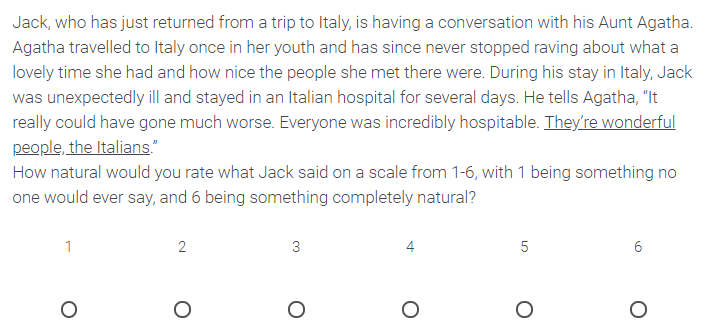
\includegraphics[width=0.8\textwidth]{EXPERIMENT_SCREENSHOT}}
\caption{Screenshot of the response task}
\label{screenshot}
\end{figure}

At the end of the experiment, participants filled out a demographics questionnaire, which asked their age, their gender, what region(s) of the UK they'd grown up in, and whether they grew up speaking any language(s) other than English. They were then given a space to include any comments or questions about the survey.

\subsubsection{Data Exclusion}

Sentences and contexts were designed in such a way that the non-dislocated target sentences in Agree contexts should be judged to be acceptable. Each sentence and context was run by a native British English speaker who did not participate in the survey to ensure they were gramatical and felicitous. However, as can be seen in Figure \ref{itemNDa}, item 5, `That was a tasty dish,' and item 6, `That rosé was a good wine,' both have mean acceptability ratings of less than 4. A mean that low for the non-dislocated sentence in the Agree context is a sign of a problem inherent to those individual sentences or contexts, and their low acceptability even in this case makes them unsuitable for measuring the effects of right dislocation on the acceptability of these utterances in context. Thus, the responses to all variants of items 5 and 6 have been excluded, leaving 6 items remaining.

\begin{figure}[hbt]
\centering
\fbox{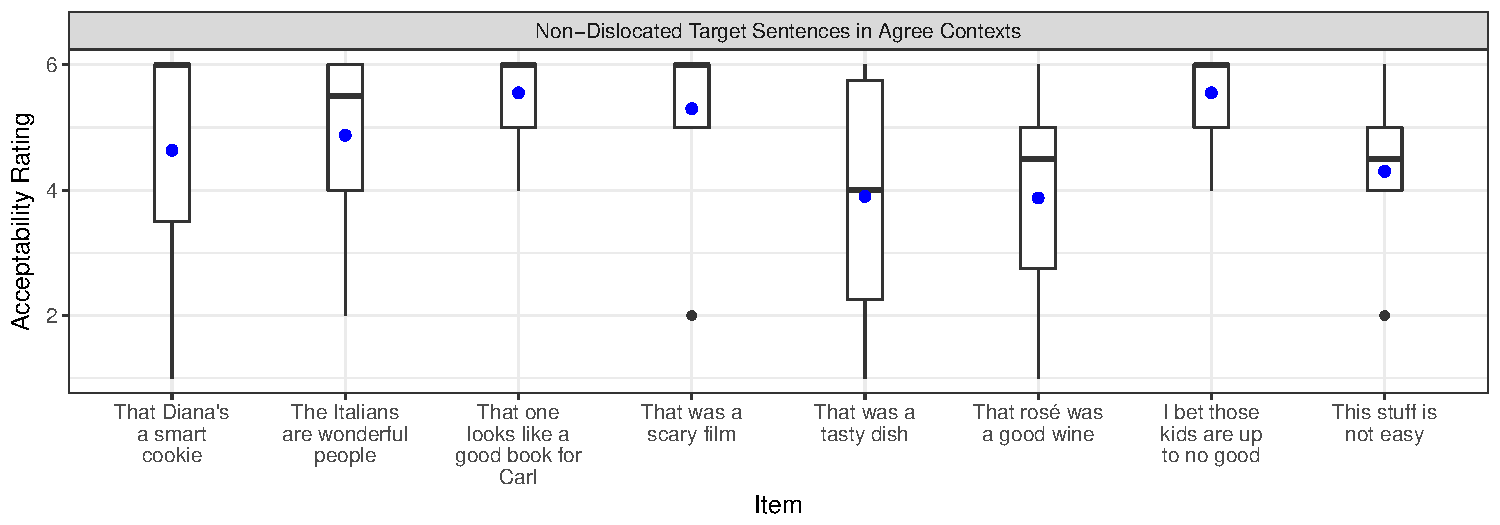
\includegraphics[width=\textwidth]{OFFICIAL_per_item_aND.pdf}}
\caption{Boxplot of acceptability ratings for non-dislocated target sentences in Agree contexts for each item. Blue dots indicate means and notches indicate medians.}
\label{itemNDa}
\end{figure}

\subsection{Results \& Discussion}

If my hypothesis is correct and right dislocation is less acceptable when the speaker does not expect the hearer to agree with the propositional content of the utterance, we would expect right-dislocated target sentences to receive significantly lower acceptability ratings in Disagree contexts than in Agree contexts. Additionally, this difference would have to be larger than any difference between the acceptability ratings of non-dislocated target sentences in these contexts, in order to ensure that participants don't find \emph{all} target sentences equally less acceptable when the speaker expects the hearer to disagree with them. 

Figure \ref{fig:predres} shows roughly what the results of this experiment would be predicted to be based on my hypothesis: with right-dislocated target sentences receiving much lower acceptability ratings in Disagree contexts than in Agree contexts, to a greater degree than the difference in acceptability ratings for non-dislocated target sentences in these contexts. The absolute difference between non-dislocated and right-dislocated variants is irrelevant to this hypothesis -- what matters is the difference in the size of the difference between Agree and Disagree contexts for right-dislocated target sentences versus non-dislocated target sentences.

\begin{figure}[bth]
\centering
\subfloat[Predicted results]{\fbox{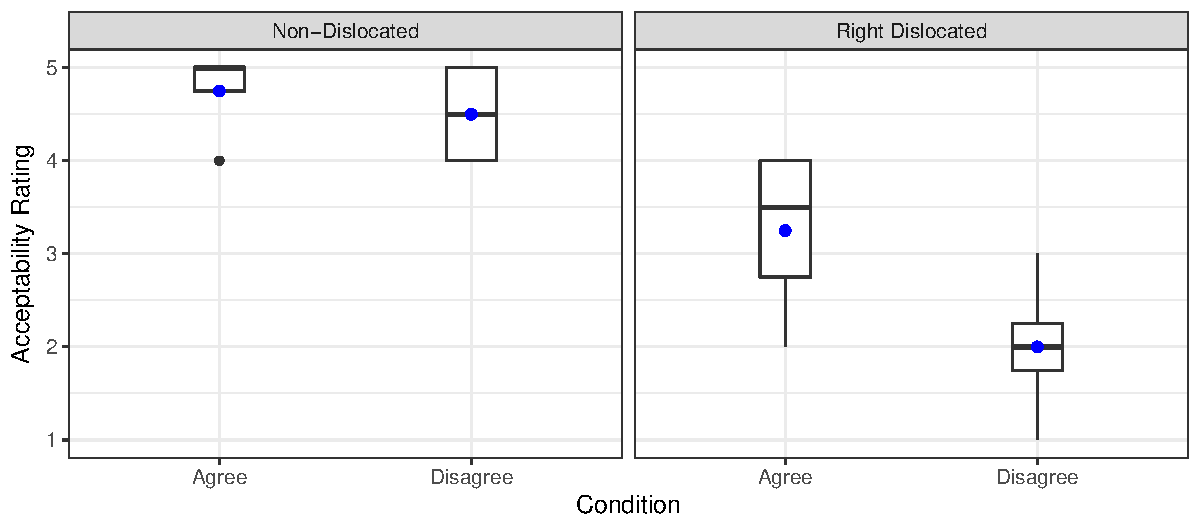
\includegraphics[width=0.8\linewidth]{OFFICIAL_fake_prediction.pdf}}\label{fig:predres}}
\hfill
\subfloat[Actual results]{\fbox{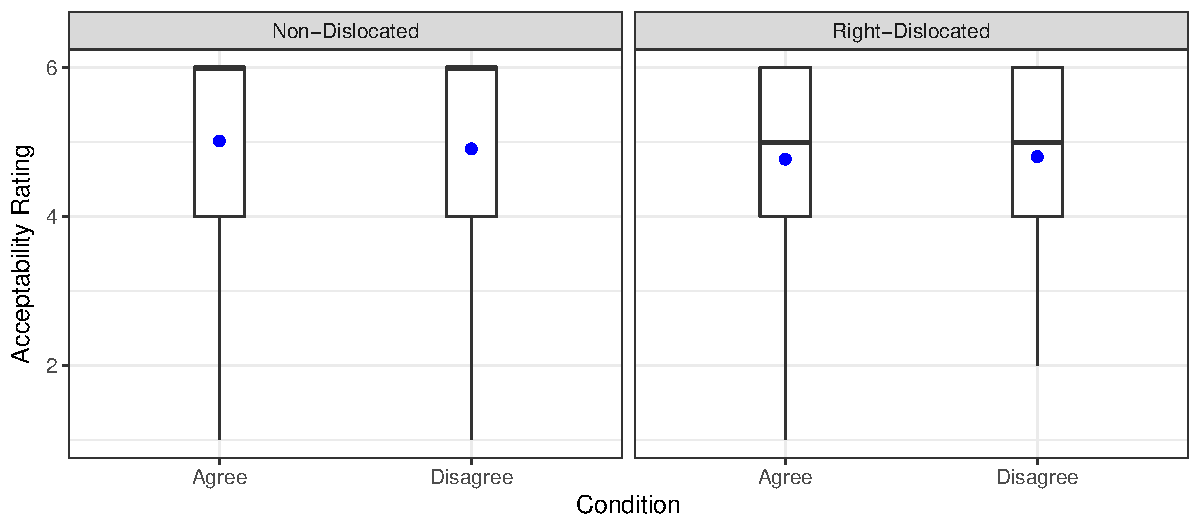
\includegraphics[width=0.8\linewidth]{OFFICIAL_per_type.pdf}}\label{fig:actres}}
\caption{Boxplots of predicted and actual acceptability ratings by condition}
\label{bytype}
\end{figure}

The actual results of the experiment differ from these predictions. As can be seen in Figure \ref{fig:actres}, while right-dislocated sentences are considered somewhat less acceptable than non-dislocated sentences across all contexts, the context had no effect on the acceptability judgments for either target sentence variant. These findings do not support the hypothesis that right dislocations are more acceptable when the speaker expects the hearer to agree with the proposition expressed by the dislocated utterance.

Given how far this departs from my predictions, it is worthwhile to investigate why the experiment did not find support for my hypothesis by reviewing the the results in more detail. In particular, I looked at inter-participant, regional, and inter-item variation for more information.

%The hypothesis described at the beginning of this section predicts that right dislocated clauses would be, on average, less acceptable in Disagree contexts than in Agree contexts, more so than a non-dislocated clause. As can be seen in Figure \ref{bytype}, there is minimal difference in both the medians and the means of the non-dislocated clauses in Agree vs. Disagree contexts. This assuages any concerns that any difference seen between Agree and Disagree contexts among right dislocations is due solely to participants' dislike for disagreement. Right dislocated sentences are on the whole less acceptable than non-dislocated sentences, which is to be expected given the colloquial spoken-English nature of right dislocation constructions. However, upon looking at the data for right dislocated sentences, it appears that there is also minimal difference between the Agree and Disagree contexts here as well. These findings do not support the hypothesis that right dislocations are more acceptable when the speaker expects the hearer to agree with the proposition expressed by the dislocated utterance.

\subsubsection{Inter-participant Variability}

\begin{figure}[bt]
\centering
\noindent
\makebox[\textwidth]{%
\fbox{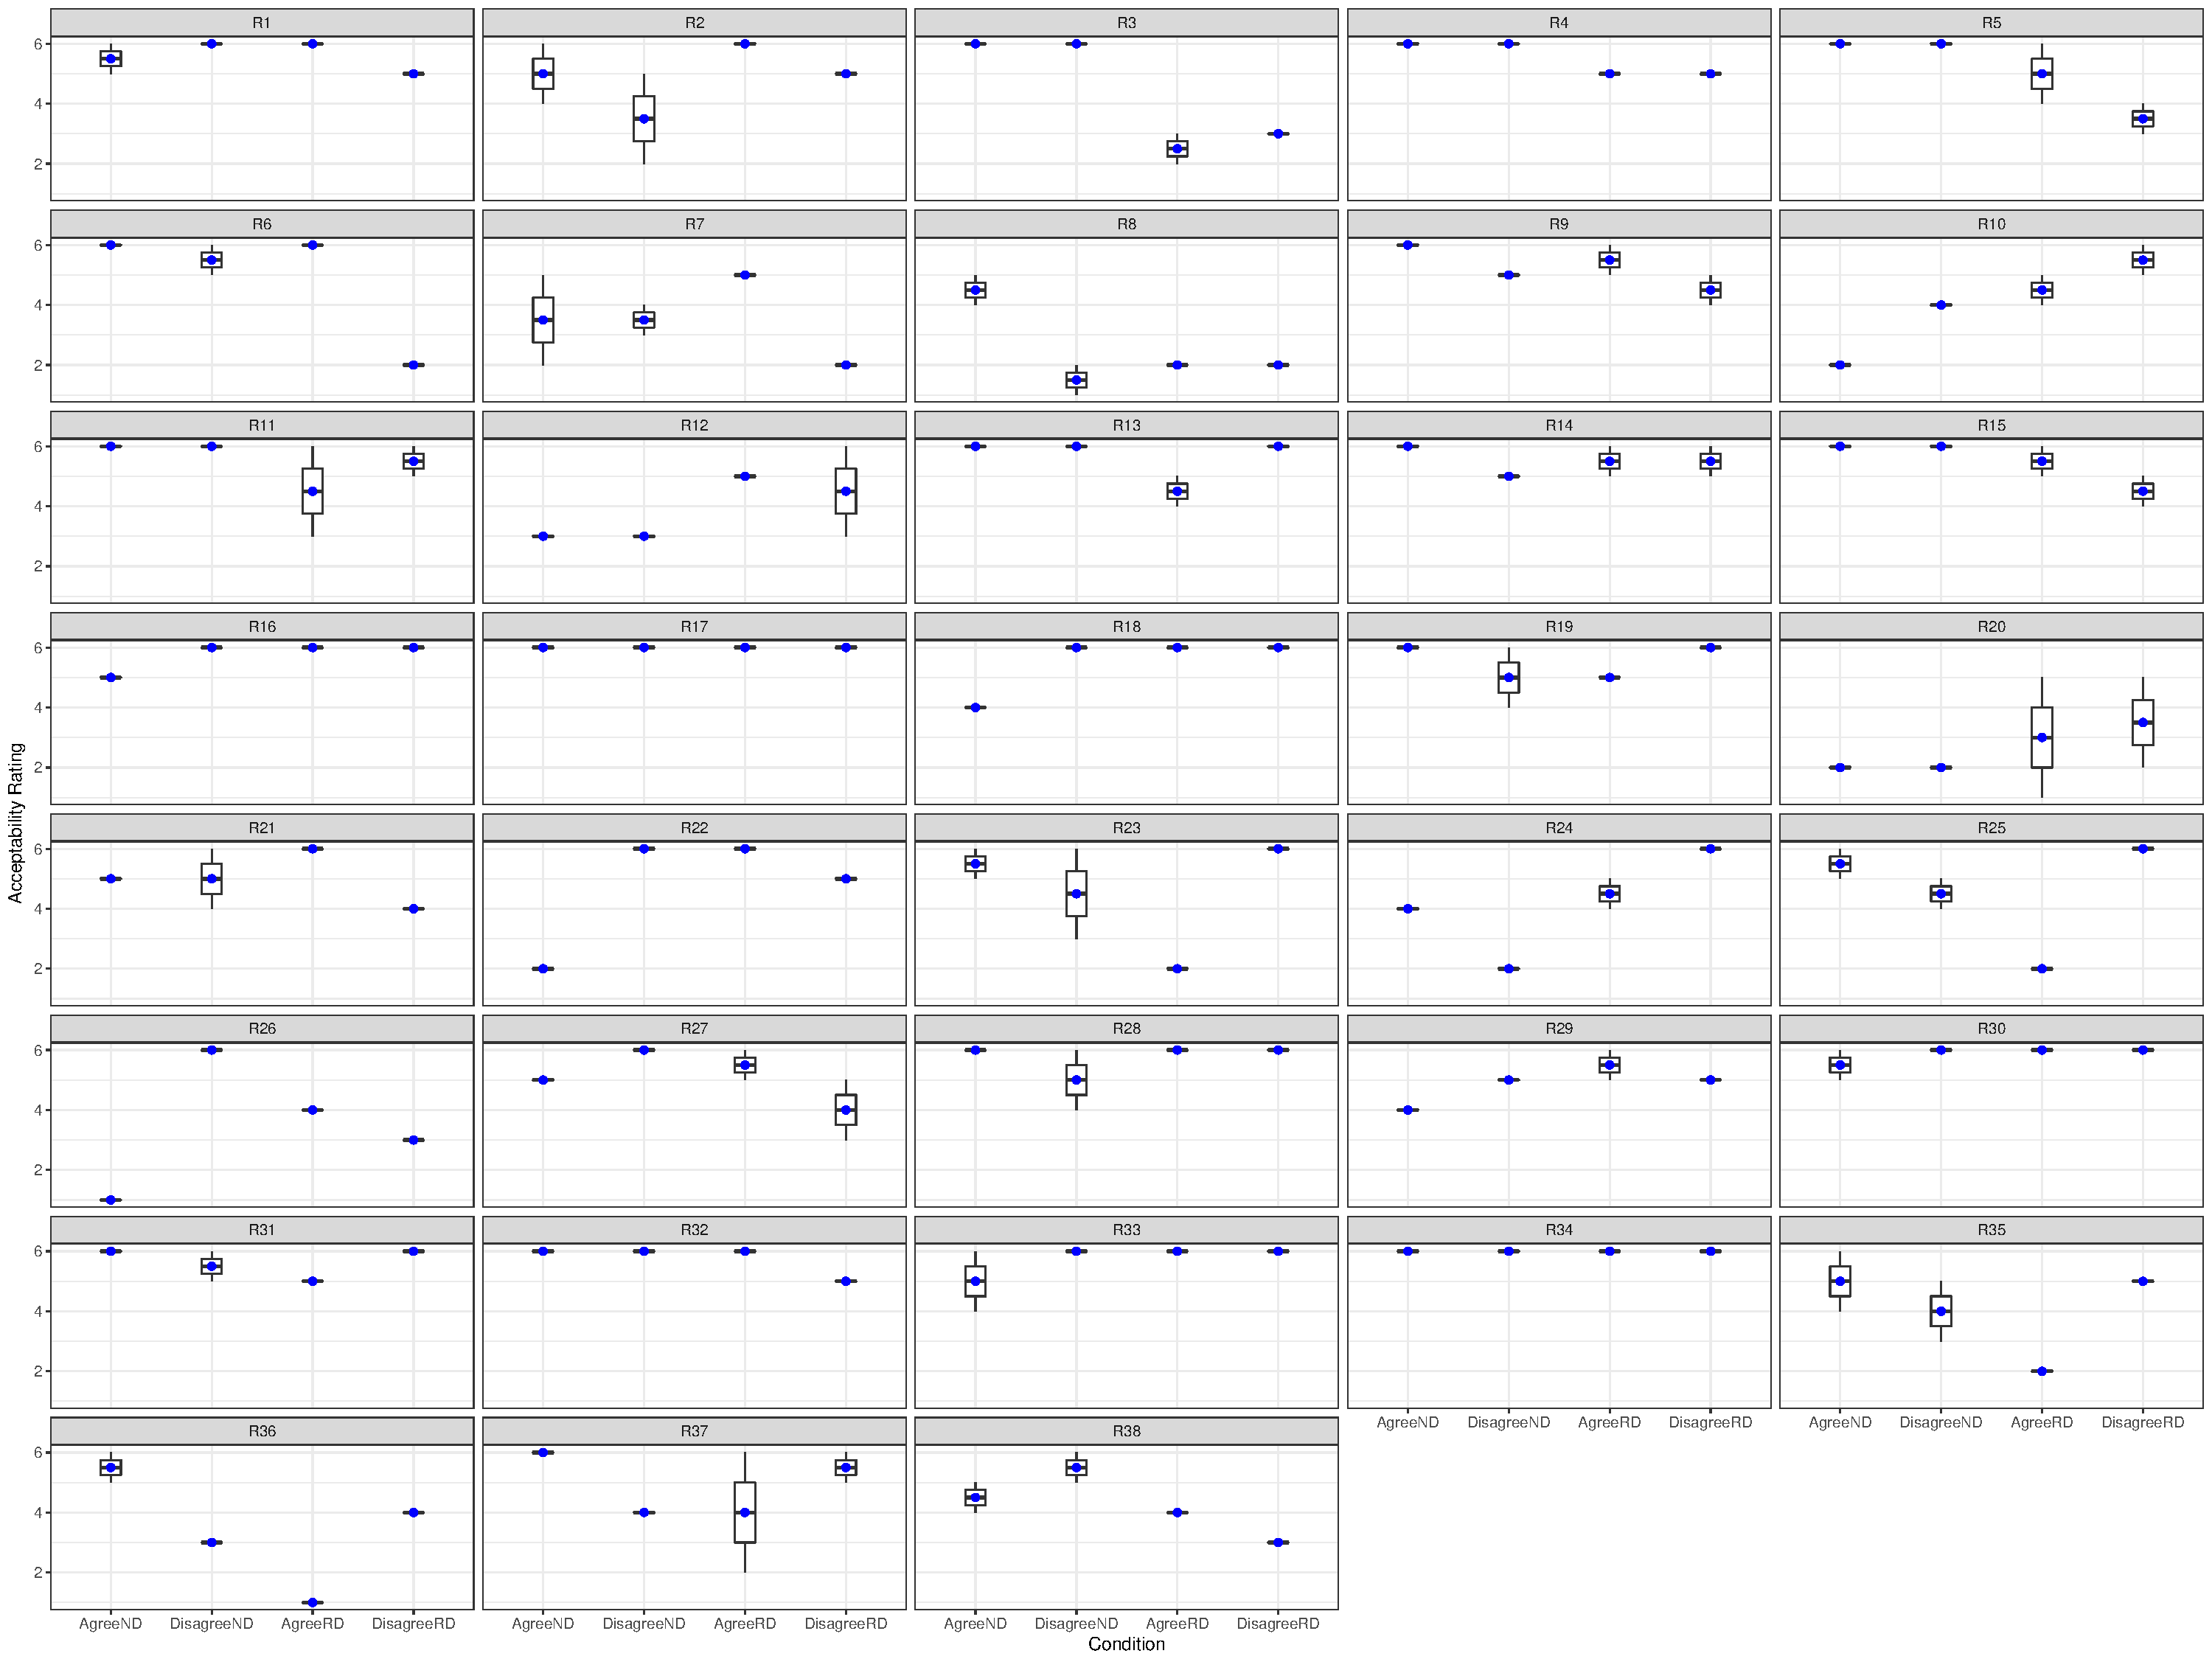
\includegraphics[width=1.1\textwidth]{OFFICIAL_per_participant_2.pdf}}}
\caption{Boxplot of acceptability rating by condition and participant}
\label{bypart2}
\end{figure}

When each participant's data is looked at separately, quite a bit of variability appears. As can be seen in Figure \ref{bypart2}, several very different patterns of responses occur among the participants. Several participants' responses do fit the pattern predicted by my hypothesis, with a lower mean acceptability for right dislocations in the Disagree than in Agree contexts (R5, R6, R7, R21), while many others exhibited the opposite pattern, with strikingly lower mean acceptability in the Agree contexts (R10, R13, R23, R24, R25, R35, R36). Another interesting observation is a number of the participants' (R7, R10, R22, R26) distaste for non-dislocated sentences in Agree contexts -- what should theoretically be the most acceptable, unmarked version. A relatively large number of the participants had quite low mean acceptability for this condition in particular. My hypothesis does not predict this.

A potential explanation for some of this variance is the experiment's lack of control for irony. To quote a comment one participant left upon completing the experiment: ``We British can say ANYTHING with a sarcastic tone and invert the meaning, and we like to do that A LOT!'' Another participant commented, regarding a particular item, that ``If she's saying this tongue-in-cheek (very British) then the appropriateness is higher than if she's being sincere." Since the survey made no attempt to control for these sorts of ironic, tongue-in-cheek comments, it was left up to individual participants to essentially guess at the sincerity of any edge cases, which could lead to the high amount of variation we see here.

\subsubsection{Regional Variability}

Though these types of NP-only right dislocations have not been described as particularly localized or regional in the existing literature, a number of participants made comments regarding the regional nature of these right dislocation constructions.

\begin{wrapfigure}{R}{0.5\textwidth}
 %\vspace{-5pt}
 \centering
    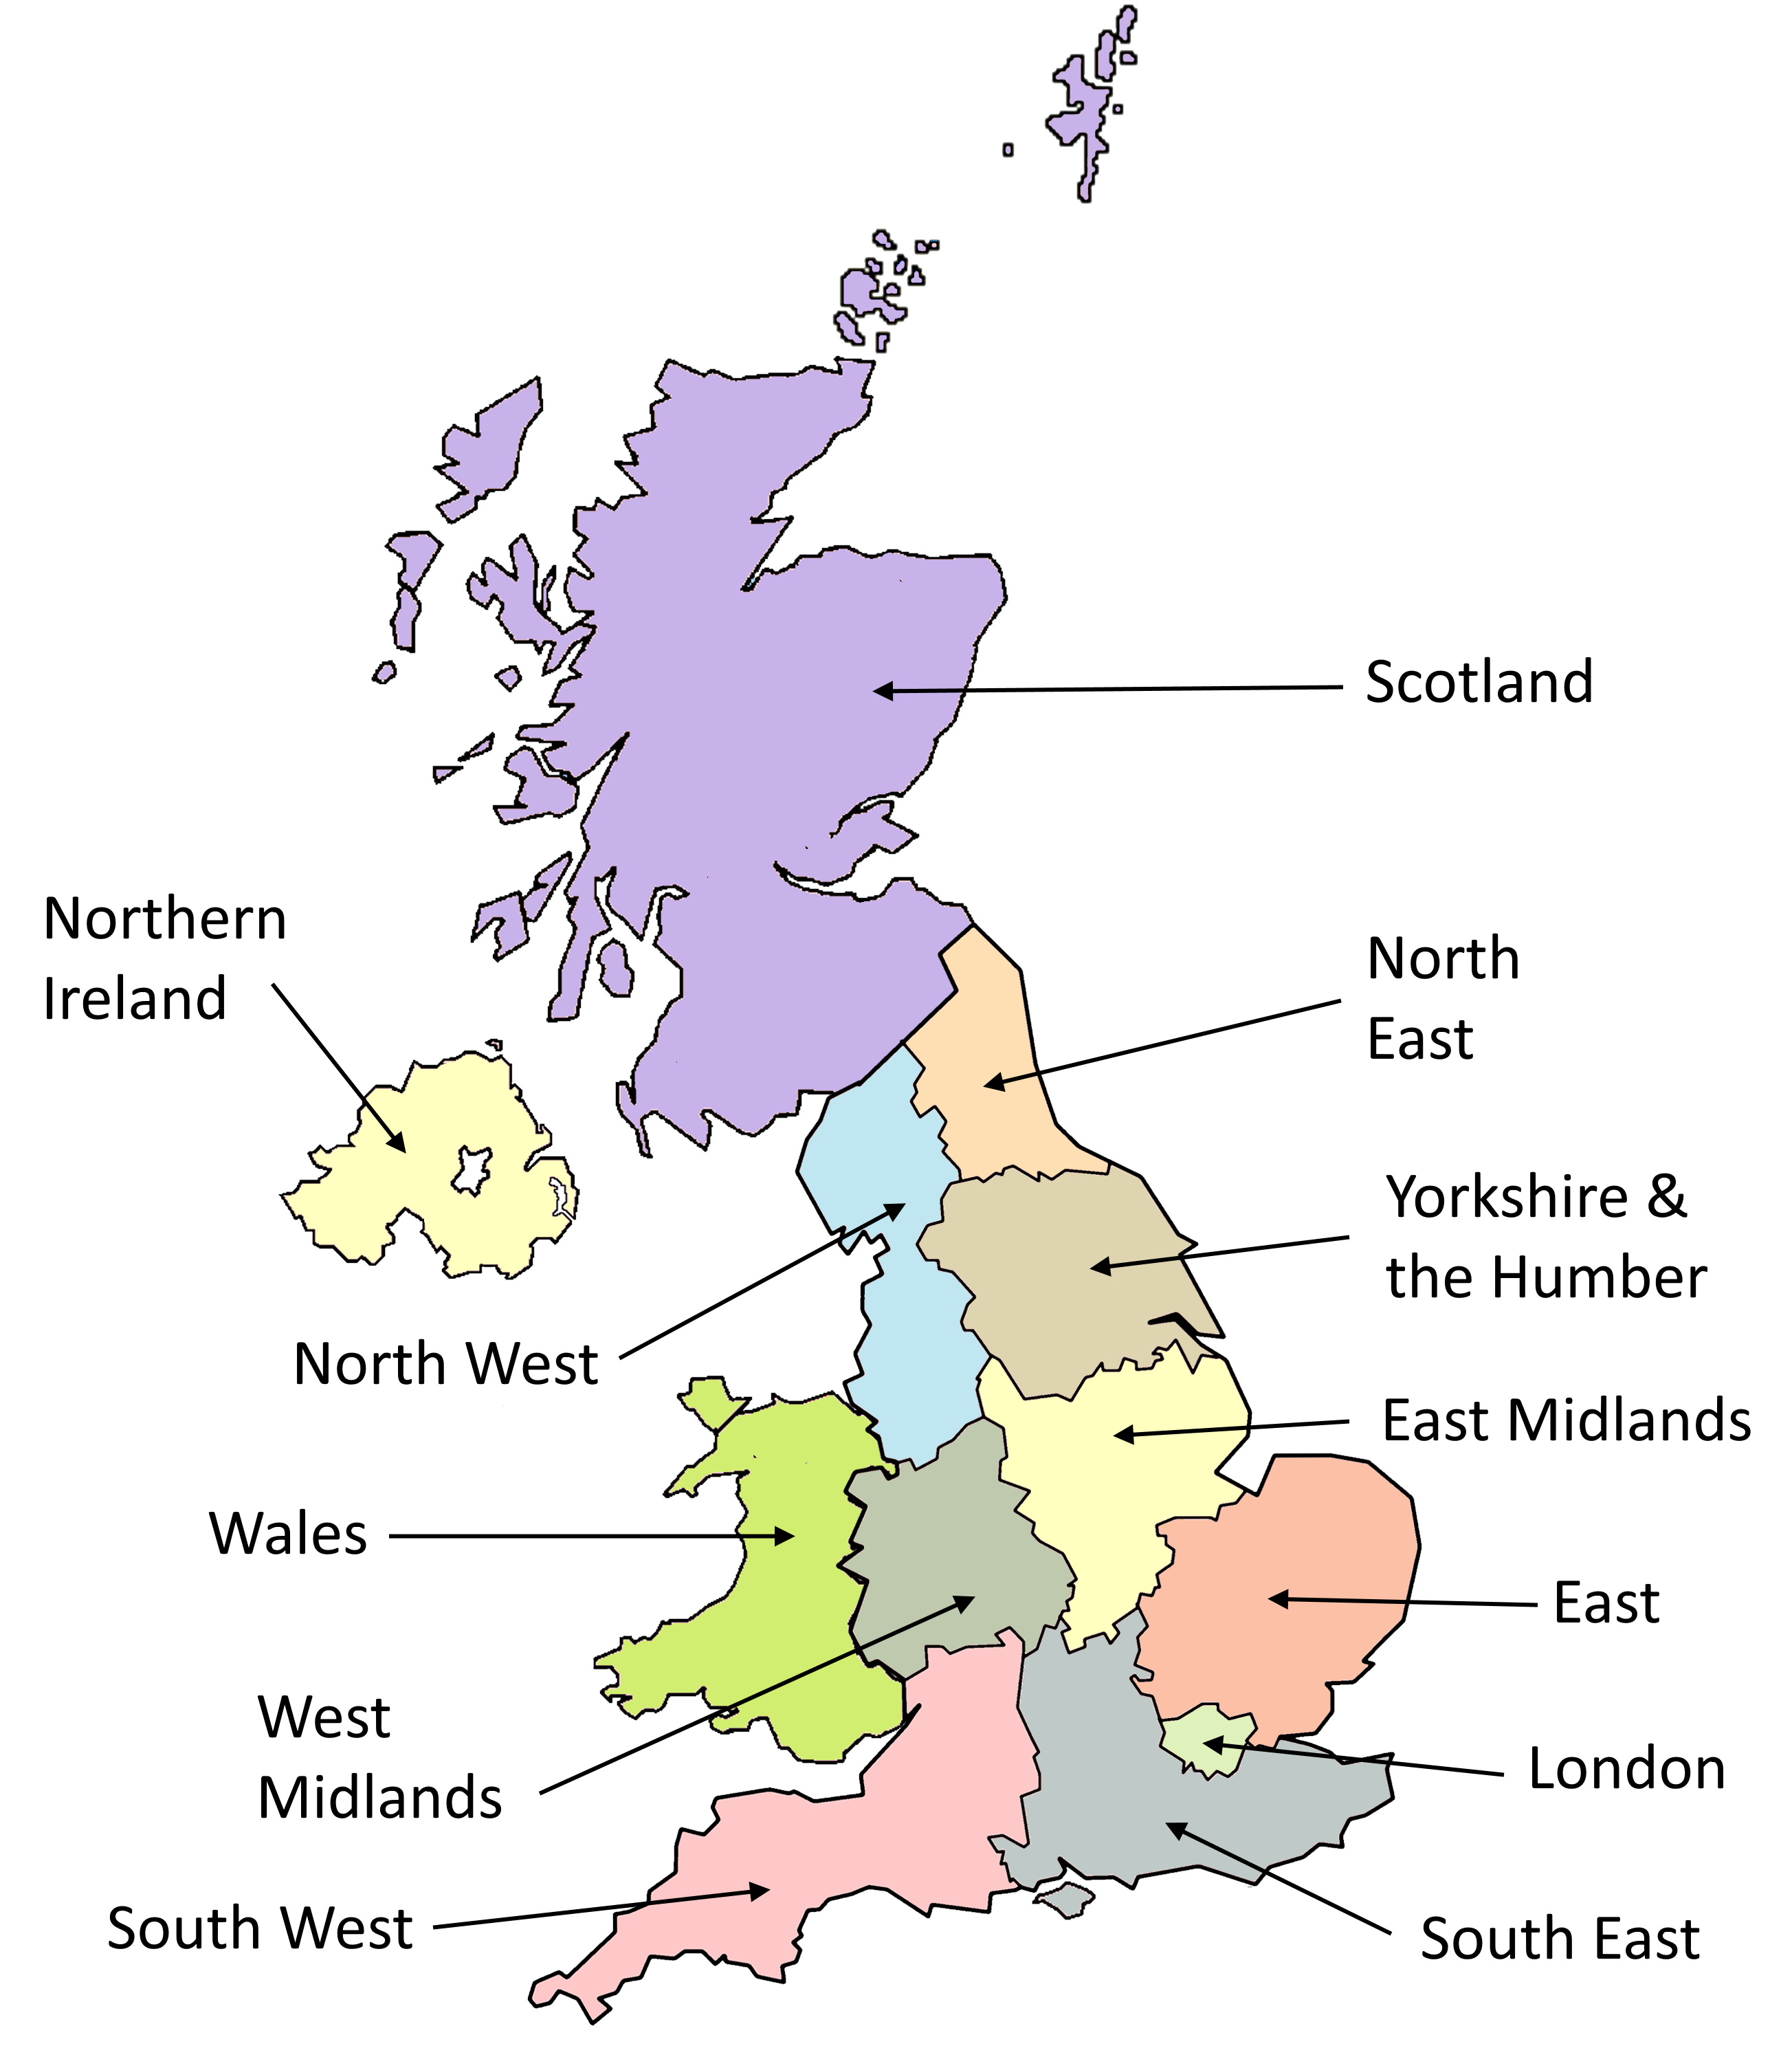
\includegraphics[width=0.44\textwidth]{United_Kingdom_NUTS_1_B.png}
  \caption[Map of NUTS 1 regions in the UK]{Map of NUTS 1 regions in the UK\protect\footnotemark}
%  \footnotesize Retrieved from 
      \label{map}
\end{wrapfigure}
\footnotetext{Based on image by Piccolo Modificatore Laborioso at English Wikipedia.}

One participant commented, ``Perhaps it's my working class background (bottom of the social pile, right here!)/time spent around people with thick Yorkshire accents, but some of the phrases which sounded quite natural to me might be somewhat alien to my social betters - as far as I'm aware, folk from London don't tend to add `That one' to their speech as much?'' and another wrote that, ``Ending sentences with ` , that one' or `those kids' is a lot more common in the north of England, compared to the south.'' Based on this, one might expect judgments of right dislocations' acceptability to differ based on the region in which the participant grew up.

In the demographics portion of the survey, participants were asked to report where in the UK they grew up. Their responses were then sorted into their first-level subdivisions according to the Classification of Territorial Units for Statistics (NUTS), shown in Figure \ref{map}. Of the 38 participants, 7 reported growing up in the North West of England, 7 in Yorkshire and the Humber, 6 in the South East, 5 in the East, 4 in the West Midlands, 3 in the South West, 2 in the North East, 1 each in the East Midlands, Scotland, and Wales. The regions with only one participant each are combined into `Other' in Figure \ref{byreg}. 

\begin{figure}[htb]
\centering
\noindent
\makebox[\textwidth]{%
\fbox{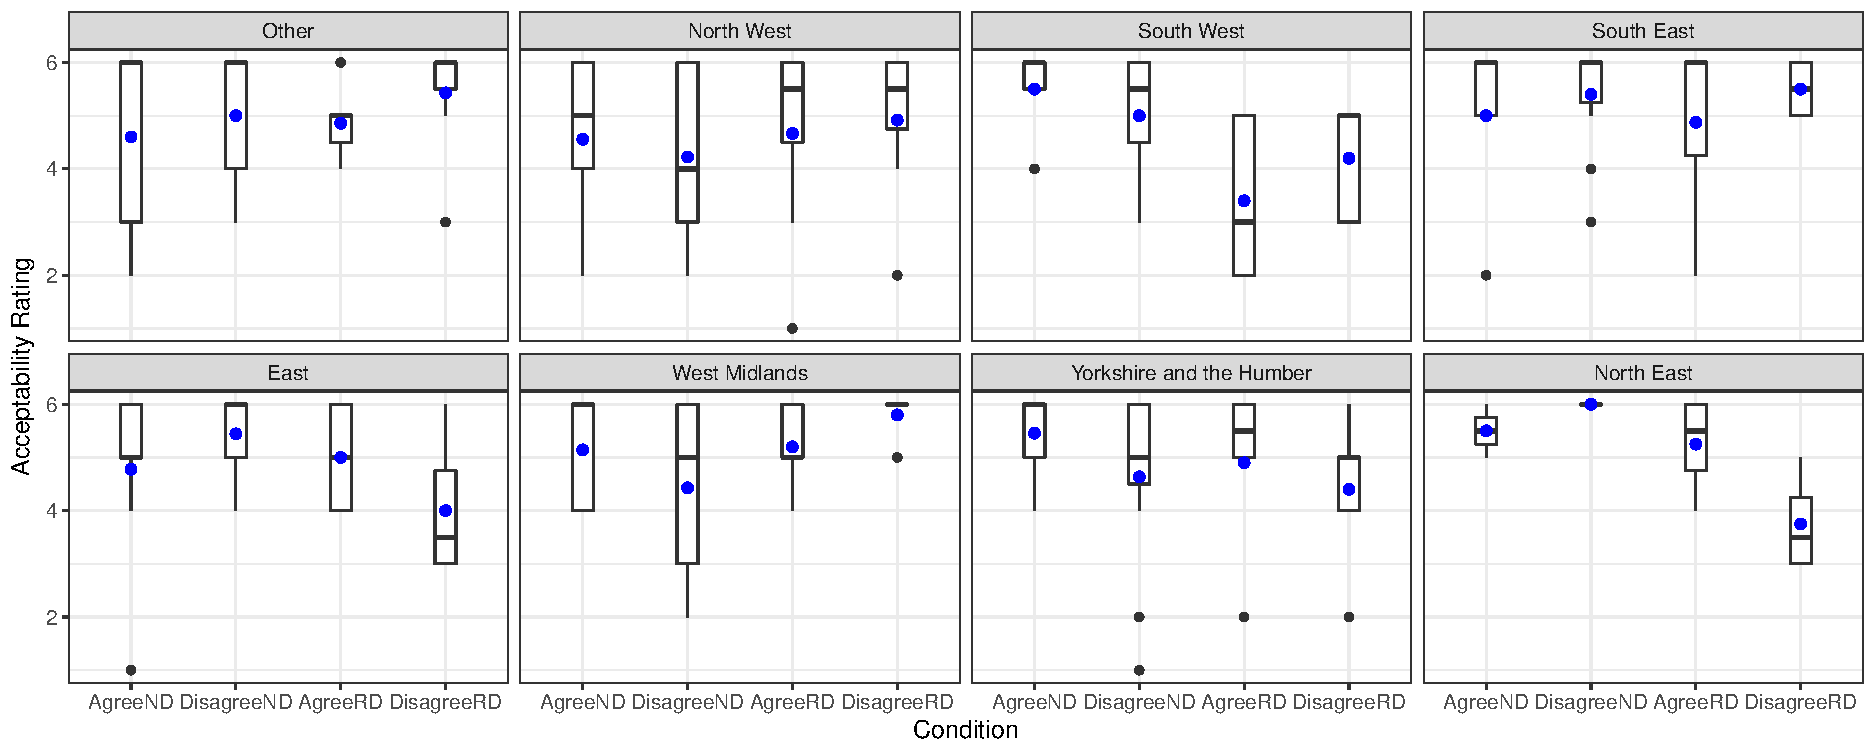
\includegraphics[width=1.1\textwidth]{OFFICIAL_per_region_1.pdf}}}
\caption{Boxplot of acceptabiliy rating by condition and NUTS 1 region}
\label{byreg}
\end{figure}

As Figure \ref{byreg} shows, there are indeed differences in responses based on the region in which participants grew up. Speakers who reported growing up in the East, North East, and Yorkshire and the Humber appear to indeed find right dislocations more acceptable in Agree contexts than in Disagree contexts, as predicted by my hypothesis. This is not the case for speakers from other regions of the UK. Additionally, speakers from the South West appear to find right dislocated constructions markedly worse than speakers from other regions. It is possible that non-ironic use of right dislocation is indeed associated with an expectation on the part of the speaker that the hearer readily agree with the content of the utterance, but that this only holds for speakers from regions that use such utterances more often in everyday speech, while speakers from regions where such utterances are less often used are more likely to interpret the marked right dislocation pattern as a sign of irony or sarcasm. 
However, given the small sample size for certain regions (the North East and South West in particular), these results should all be taken with a grain of salt until further research into the varying attitudes toward these constructions by region can be conducted.

\subsubsection{Inter-Item Variability}

Though there was little difference between the acceptability judgments of right-dislocated target sentences in Agree versus Disagree contexts, that does not necessarily hold for each individual item. It is possible that some of the items showed higher acceptability in Agree contexts while others showed higher acceptability in Disagree contexts, thus cancelling each other out when the data was viewed as a whole. If this is the case, it is worthwhile to check whether any individual items behaved as predicted and whether those that did or those that did not have anything notable in common.

%While overall, there was little difference between right dislocations in Agree and Disagree contexts, there was quite some difference for some items -- however, as can be seen in Figure \ref{byit}, certain items showed higher acceptability in the Agree context than in the Disagree context while others showed the opposite effect. Thus, the differences cancelled each other out when looking at the data as a whole. Is it possible that the sentences and contexts that behaved similarly to what was predicted by the hypothesis have something notable in common? 

\begin{figure}[bth]
\centering
\fbox{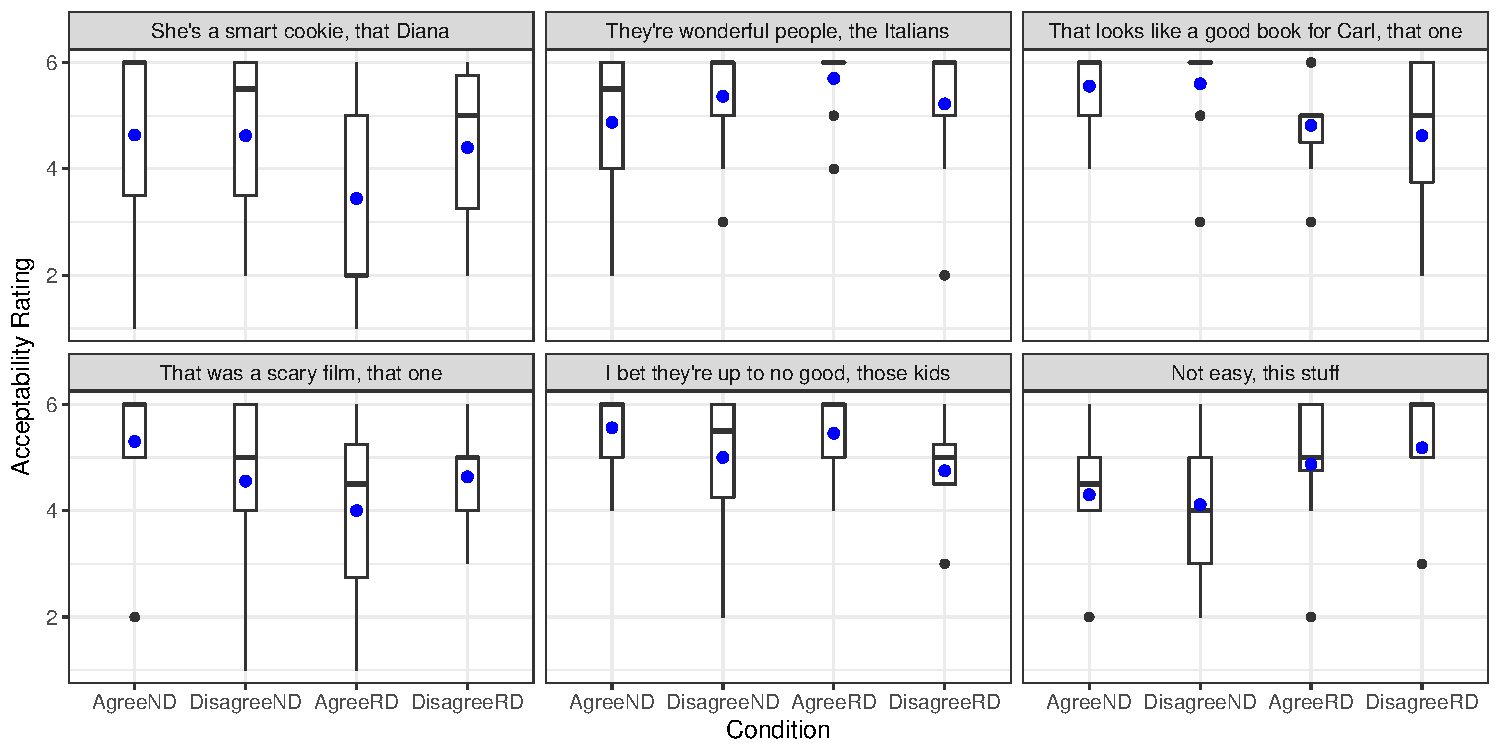
\includegraphics[width=\textwidth]{OFFICIAL_per_item_1.pdf}}
\caption{Boxplot of acceptability rating by condition and item}
\label{byit}
\end{figure}


As one can see in Figure \ref{byit}, for some items the right-dislocated target sentences are considered more acceptable in Agree contexts than in Disagree contexts, whereas the opposite is true for other items. Though these differences are smaller for some items than others, it may be worthwhile to look at those items for which Agree or Disagree contexts are more obviously preferred.

\begin{multicols}{2}
\samepage
Agree-preferred:
\begin{itemize}
    \item They're wonderful people, the Italians.
    \item I bet they're up to no good, those kids.
\end{itemize}\vfill\null
\columnbreak
Disagree-preferred:
\begin{itemize}
    \item She's a smart cookie, that Diana
    \item That was a scary film, that one.
    \item Not easy, this stuff
\end{itemize}
\end{multicols}

Those for which participants exhibited the greatest preference for the Agree contexts when it came to right dislocations, items 2 and 7, were the only two items in which the right-dislocated NP had a group referent: \textit{the Italians} and \textit{those kids}. Research has shown that that use of determiners like \textit{the} and \textit{those} with groups can introduce a distancing effect (see \citealt{acton2014pragmatics}), and demonstratives in particular do occur disproportionately often in right dislocations. 
It is possible that these effects are creating or amplifying any tendency for right dislocation to correspond to the speaker's expectation that the hearer agree with them. However, further research needs to be done to truly investigate the connection between right dislocations and such determiners, if any.

It is also possible that the relationship between the speaker and the hearer influenced acceptability of right dislocation. In items 2 and 7, the context involves speaking to an older female relative in an informal context, whereas this is not the case for items 1, 3, 4, and 8 -- item 1 involves two colleagues in a vaguely professional context, item 3 a wife speaking to her husband, item 4 a father speaking to his son, and item 8 two adult brothers. While it seems unlikely that right dislocation serves to mark a speakers expectation that the hearer agree with the proposition expressed by the utterance only when the hearer is an older female relative, it is possible that there is some relationship between speaker-hearer intimacy and whether right dislocation is licensed. Perhaps this could be an explanation for the variance seen here. Further research would be necessary to investigate whether there is any merit to this pattern.

\subsection{Summary}

When presented with right-dislocated and non-dislocated target sentences in Agree and Disagree contexts, participants did not prefer Agree contexts to Disagree contexts for either right-dislocated or non-dislocated target sentences. These findings do not support my hypothesis that right dislocation is less acceptable when the speaker expects the hearer to agree with the propositional content of the right-dislocated utterance. 

Several  weak points in the study design could be responsible for the failure of this experiment to find support for my hypothesis. Failure to control for irony due to the textual presentation of the target sentences may have had a large effect on these result; they would likely have been very different if audio stimuli were used. Additionally, a larger sample of British English speakers, with more from each area within the UK, could provide more information about whether right dislocation's meaning and use differs by region. Furthermore, differences in factors like the specificity the dislocated NP and the use of definite versus demonstrative determiners introduced variability that may have obscured any effects of right dislocation.

While these results are largely inconclusive in and of themselves, hopefully they can serve as a good starting-point for further research into right dislocation and its discourse functions in the future.

%When presented with right-dislocated and non-dislocated sentences in Agree and Disagree contexts, participants did not prefer Agree contexts to Disagree contexts for either right-dislocated or non-dislocated target sentences. While these findings do not support the hypothesis that right dislocation is more acceptable in contexts wherein the speaker expects the hearer to agree with the propositional content of the right-dislocated utterance, several weak points in the study design have revealed potential routes for future research. Use of right dislocations ironically has not been studied, but seems to play a large role in its use, and a larger sample of British English speakers from a greater variey of areas within the UK could illuminate whether right dislocation has social meaning that differs by region. Furthermore, even though right dislocation does not appear to be a marker of speaker-hearer agreement, it may influence other indicators of speaker-hearer solidarity; this should be explored in future research as well.

\section{Conclusion} \label{conclude}

At the very least, right dislocation is a versatile construction with several overlapping discourse functions. While some of its uses are relatively well-understood, others sorely need further research. In particular, discourse functions outside of afterthoughts, epithets, and information structure have lacked in-depth research. This thesis sought to contribute some such research by experimentally testing whether right dislocation is more acceptable when the speaker expects the hearer to agree with the propositional content of the utterance. The results of the experiment do not support this hypothesis, but this leads us to further questions to be answered in future research.

One glaring flaw in this experiment was its failure to control for irony. A follow-up experiment using auditory stimuli to manipulate whether participants perceive the right dislocated sentence as ironic would provide insight, as would further thought on how best to control for irony in the first place. Whether a right dislocation is more likely to be ironic than its non-dislocated counterpart is also worth discussing. If right dislocations are particularly suited to ironic use as the comments made by participants seem to imply, one must wonder why this is the case. Are these constructions indeed more often used ironically than not? If so, is it possible that right dislocations have some sort of emphatic property, thereby lending themselves better to sarcasm, or is there some other reason that this construction in particular is so often used ironically? These are questions worth addressing in future research. 

Additionally, other claims made in \citealt{aijmer_themes_1989} merit future research. In addition to claiming that right dislocation is used when the transmission of information is not important and there is already common ground, \citeauthor{aijmer_themes_1989} claims that right dislocations are used to create intimacy and affection between the speaker and the hearer. If this is the case, it may explain the variation seen between items in this experiment, as participants may have considered the creation of intimacy and affection between the speaker and hearer more or less appropriate in some contexts than in others.

The connection to affective demonstratives and particularly to `that' is also worth further exploration. It is unlikely that the high frequency of demonstrative use in right-dislocated NPs and in particular distal demonstrative use is a coincidence. In addition to potentially fostering the intimacy between speaker and hearer described in \citealt{aijmer_themes_1989}, demonstrative use could indicate that right dislocation is associated with a physical or emotional distancing between the speaker or hearer and the referent of the dislocated NP. More research into how exactly right dislocation and demonstratives are connected is definitely needed.

The apparent association of right dislocation with Northerners and the working class also merits further research. While related constructions like the `expanded right dislocation' and `reverse right dislocation' described in \citealt{durham_right_2011} have been described as particular to dialects in certain Northern regions, the `standard' right dislocation investigated in this paper has not been described as particularly Northern. Though some (\citealt{visser_historical_1963}, \citealt{aijmer_themes_1989}) refer to the construction as `dialectical' or `regional' in passing, they do not specify it as belonging to any region in particular. If even these right dislocations are considered especially Northern by our participants, it would be worth investigating whether these right dislocations and other similar constructions are indeed used more often in the North and whether they are being used to project a sort of Norther, working-class persona on the part of the speaker.

Finally, right dislocations do appear to bear at least a superficial similarity to tag questions (e.g., ``That Diana's a smart cookie, isn't she?''), but they do not appear to have been viewed in parallel or compared with one another in any existing literature. This is particularly true when it comes to the `expanded' and `reverse' forms from \citealt{durham_right_2011}, which even more closely resemble tag questions - they have even been referred to as `tag statements' in the past (such as in \citealt{melchers_its_1983}). A comprehensive look at the relationship between `standard' right dislocation, those alternate forms, and tag questions has the potential to be extremely informative.


%Until now, research into right dislocation's social meaning was pretty much limited to a few lines in passing in the occasional paper, with little experimental evidence to back any of it up. \citeauthor{aijmer_themes_1989}'s (\citeyear{aijmer_themes_1989}) claim that right dislocation serves as a mark of speaker-hearer solidarity is by far the most concrete explanation in the literature, but the results of this experiment do not seem to support that analysis. If right dislocation is a mark of speaker-hearer solidarity, one would have expected right dislocation to be associated with the speaker's higher expectation that the hearer agree with their utterance than in a non-dislocated clause, but that does not seem to be the case given these results. 

%This experiment's failure to control for irony could be to blame for these results. But if that is the case, what is the best way to control for irony in future experiments like this? More importantly, do participants prefer these constructions when used ironically because they have emphatic properties, or for some other reason? Further exploration into the use of these constructions ironically would be extraordinarily useful.

%It is also possible that a speaker's expectation that the hearer agree with them is not a good metric for speaker-hearer solidarity. Other ways of measuring speaker-hearer solidarity should be investigated. In particular, looking into the perceived distance between the speaker and the hearer, as well as the speaker and the referent of the right-dislocated NP, would be a good next step to investigate when it comes to the claim that right dislocations mark speaker-hearer solidarity.

%While these results are largely inconclusive in and of themselves, they reveal a number of avenues that simply have not been sufficiently explored in regards to right dislocation's social function in discourse. Hopefully this experiment will serve as a starting-point for future research into the social meaning of these and other interesting constructions.

\section{Acknowledgements}

This work was partially supported by an Arts and Sciences Undergraduate Research Scholarship and an Arts and Sciences International Research Grant. I would like to thank Hannah de Vries and everyone else at the University of York for their hospitality while I was in Yorkshire and their help reaching potential participants, as well as Agata Renans for helping get me in touch with them in the first place. I would also like to thank Peter Stannard for helping me build target sentences and contexts and Lucille Blumire for help with UK geography.

I would also especially like to thank Lauren Squires for serving on my thesis committee and providing excellent insight on this thesis. Last but not least, I would like to thank my advisors, Marie-Catherine de Marneffe and Judith Tonhauser, for their neverending support and patience throughout this project. I could nev

\newpage
\begin{appendices}
\section{List of All Items} \label{alladem}

\begin{enumerate}
\footnotesize
    \item [Item 1:] \hfill
    \begin{enumerate}
        \item [Agree:] Diana is a first-year grad student who is presenting her research to the professors in her department. One of the professors, Dr.\ Smith, is very easily pleased when it comes to new students' work and always gives the students positive comments on even fairly mediocre presentations. After Diana leaves, another professor, Dr.\ Brown, approaches Dr.\ Smith and says,
        \item [Disagree:] Diana is a first-year grad student who is presenting her research to the professors in her department. One of the professors, Dr.\ Smith, has very high expectations of new students and tends to be incredibly critical of their work, criticizing even the best of presentations. After Diana leaves, another professor, Dr.\ Brown, approaches Dr.\ Smith and says,
        \begin{itemize}
        \setlength{\itemindent}{5em}
            \item [ND:] ``That Diana's a smart cookie.''
            \item [RD:] ``She's a smart cookie, that Diana.''
        \end{itemize}
    \end{enumerate} 
    \item [Item 2:] \hfill
    \begin{enumerate}
        \item [Agree:] Jack, who has just returned from a trip to Italy, is having a conversation with his Aunt Agatha. Agatha travelled to Italy once in her youth and has since never stopped raving about what a lovely time she had and how nice the people she met there were. During his stay in Italy, Jack was unexpectedly ill and stayed in an Italian hospital for several days. He tells Agatha, ``It really could have gone much worse. Everyone was incredibly hospitable.
        \item [Disagree:] Jack, who has just returned from a trip to Italy, is having a conversation with his Aunt Agatha. Agatha travelled to Italy once in her youth and has since never stopped complaining about how rudely she was treated there. During his stay in Italy, Jack was unexpectedly ill and stayed in an Italian hospital for several days. He tells Agatha, ``It really could have gone much worse. Everyone was incredibly hospitable.
        \begin{itemize}
        \setlength{\itemindent}{5em}
            \item [ND:] The Italians are wonderful people.''
            \item [RD:] They're wonderful people, the Italians.''
        \end{itemize}
    \end{enumerate}
        \item[Item 3:]\hfill 
        \begin{enumerate}
        \item [Agree:] Rosemary and her husband Geoff are out shopping for Christmas presents. Their thirteen-year-old son, Carl, is an avid reader and is particularly fond of fantasy novels. In a bookstore, Rosemary and Geoff come across a copy of Lord of the Rings, which they love but Carl hasn't read yet. Rosemary points to the book and says to Geoff,
        \item [Disagree:] Rosemary and her husband Geoff are out shopping for Christmas presents. Their thirteen-year-old son, Carl, is an avid reader and is particularly fond of fantasy novels. Geoff doesn't want Carl to read more fantasy novels. In a bookstore, they come across a copy of A Game of Thrones. Rosemary points to the book and says to Geoff,
        \begin{itemize}
        \setlength{\itemindent}{5em}
            \item [ND:] ``That one looks like a good book for Carl.''
            \item [RD:] ``That looks like a good book for Carl, that one.''
        \end{itemize}
    \end{enumerate}
    \item[Item 4:] \hfill 
    \begin{enumerate}
        \item [Agree:] Tim and his father go to watch a horror film at the cinema. Tim is a fairly timid child and tends to be a bit easily frightened. As they leave the cinema, his father remarks,
        \item [Disagree:] Tim and his father go to watch the latest \textit{Harry Potter} film at the cinema. Tim is a teenager and more of a fan of horror films, but he goes with his dad for family bonding. As they leave the cinema, his father remarks,
        \begin{itemize}
        \setlength{\itemindent}{5em}
            \item [ND:] ``That was a scary film.''
            \item [RD:] ``That was a scary film, that one.''
        \end{itemize}
    \end{enumerate}
    \item [Item 5:] \hfill \begin{enumerate}
        \item [Agree:] Billy and Gemma go on a date to their favorite restaurant for their first anniversary. Gemma's particular favorite dish the at this restaurant is the spaghetti carbonara, so they order it to share for their special occasion. After dinner, Billy says,
        \item [Disagree:] Billy and Gemma go on a date to their favorite restaurant for their first anniversary. Billy, who is feeling adventurous, orders them the chef's surprise to share. Gemma isn't a particularly picky eater, but really dislikes any type of seafood. When the dish arrives, it just so happens to contain prawns. After dinner, Billy says,
        \begin{itemize}
        \setlength{\itemindent}{5em}
            \item [ND:] ``That was a tasty dish.''
            \item [RD:] ``That was a tasty dish, that one.''
        \end{itemize}
    \end{enumerate}
    \item [Item 6:]\hfill  \begin{enumerate}
        \item [Agree:] Jeremy and Theresa are at a couple's wine tasting. Jeremy loves wine, and Theresa knows he enjoys pretty much any wine. The two of them taste a fine French rosé that is renowned as one of the best. Once they've both tasted it, Theresa turns to Jeremy and says,
        \item [Disagree:] Jeremy and Theresa are at a couple's wine tasting. Jeremy is incredibly picky and absolutely hates English wines. The two of them taste a rosé made in Sussex. Once they've both tasted it, Theresa turns to Jeremy and says,
        \begin{itemize}
        \setlength{\itemindent}{5em}
            \item [ND:] ``That rosé was a good wine.''
            \item [RD:] ``That was a good wine, the rosé.''
        \end{itemize}
    \end{enumerate}
    \item [Item 7:]\hfill \begin{enumerate}
        \item [Agree:] Sandra is visiting her elderly mother. Sandra's mother often complains to her about how the local children are a bunch of hooligans who always get into trouble. As the two of them are talking in the kitchen, Sandra sees some neighborhood kids clustered around a neighbor's car. She says to her mother,
        \item [Disagree:] Sandra is visiting her elderly mother. Sandra's mother frequently compliments the local children, telling Sandra about how helpful, kind, and well-mannered they are. As the two of them are talking in the kitchen, Sandra sees some neighborhood kids clustered around a neighbor's car. She says to her mother,
        \begin{itemize}
        \setlength{\itemindent}{5em}
            \item [ND:] ``I bet those kids are up to no good.''
            \item [RD:] ``I bet they're up to no good, those kids.''
        \end{itemize}
    \end{enumerate}
    \item [Item 8:]\hfill 
    \begin{enumerate}
        \item [Agree:] Henry and Bob are brothers and are working together to build their niece a treehouse. Henry works as a builder and has a lot of experience with construction work, while Bob works as an accountant and isn't at all used to manual labor. After a few hours of work, Henry notices that Bob is having a hard time. He turns and says to Bob,
        \item [Disagree:] Henry and Bob are brothers and are working together to build their niece a treehouse. Henry works as a builder and has a lot of experience with construction work, while Bob works as an accountant and isn't particularly used to manual labor. After a few hours of work, Bob needs to take a break. Henry has barely broken a sweat and is clearly enjoying himself. Bob turns and says to Henry,
        \begin{itemize}
        \setlength{\itemindent}{5em}
            \item [ND:] ``This stuff is not easy.''
            \item [RD:] ``Not easy, this stuff.''
        \end{itemize}
    \end{enumerate}
\end{enumerate}

%\newpage

%\section{Text of Consent to Participate} \label{consent}

%I am doing research on British English. I may publish and/or present my findings during conference presentations based on the conversations we have. I am going to ask you for your intuitions about whether sentences sound natural in particular contexts. You can skip questions that make you uncomfortable or that you don’t want to answer. Your participation will consist of completing a ten- to twenty-minute questionnaire. You will receive £3 for your participation. The general benefit of this project is an increased understanding of understudied constructions in British English. If you decide that you do not want to participate anymore, you will not lose any benefit or receive any penalty. Also, there is no risk or discomfort in participating. All of the information taken will remain confidential. Participation is voluntary and you may stop at any time without penalty or loss of benefits. May I interview you?

%\begin{center}
%    [Participant selects ``yes'' or ``no'']
%\end{center}

%or questions, concerns, or complaints about the study, you may contact, by phone or via email, Associate Professor Judith Tonhauser (Ohio Stadium East 109B, +1 614-292-7849, tonhauser.1@osu.edu) or Bethany Toma (+1 440-637-5045, toma.18@osu.edu). For questions about your rights as a participant in this study or to discuss other study-related concerns or complaints with someone who is not part of the research team, you may contact Ms. Sandra Meadows in the Office of Responsible Research Practices by phone at +1 800-678-6251 or +1 614-688-4792, or via email at the following address: meadows.8@osu.edu. If you feel that you have been harmed as a result of this study, or for questions about a study-related injury, you may contact, by phone or via email, Associate Professor Judith Tonhauser (Ohio Stadium East 109B, +1 614-292-7849, tonhauser.1@osu.edu) or Bethany Toma (+1 440-637-5045, toma.18@osu.edu).

\end{appendices}

\newpage

\bibliography{rightDislocationThesis.bib}

\end{document}